% =====================================================================
%  SIAM Journal on Financial Mathematics -- first draft.
%  Compile:  pdflatex main && bibtex main && pdflatex main && pdflatex main
%  (or: latexmk -pdf main.tex)
% =====================================================================
\documentclass[final,onefignum,onetabnum]{siamart220329}
% ---------------------------------------------------------------------
%  Packages and notation shared by all sections.
% ---------------------------------------------------------------------
\usepackage{amssymb,mathtools}
\usepackage{booktabs,array,multirow}
\usepackage{graphicx}
\usepackage[font=small,skip=6pt]{caption}
\usepackage{enumitem}
\usepackage{placeins}
\usepackage{algpseudocode}
\usepackage{pgfplots}
\pgfplotsset{compat=1.18}
\usetikzlibrary{arrows.meta,positioning,calc}
\usepgfplotslibrary{groupplots}

% ---------------------------------------------------------------------
%  Palette and plot style shared by every figure of the section.
% ---------------------------------------------------------------------
\definecolor{mainblue}{RGB}{36,78,121}
\definecolor{cJoint}{HTML}{E07A5F}     % joint training        (terracotta)
\definecolor{cStop}{HTML}{2A9D8F}      % stop-gradient (ours)  (teal)
\definecolor{cLayer}{HTML}{E9B44C}     % layerwise             (saffron)
\definecolor{cEma}{HTML}{9C89B8}       % EMA target            (lilac)
\definecolor{cFull}{HTML}{7FA7C9}      % layerwise, full budget (sky)
\definecolor{cInk}{HTML}{264653}       % reference lines, text (deep slate)
\definecolor{cGrid}{HTML}{E6EBEF}
\definecolor{cBand}{HTML}{EAF5F3}      % light teal band
\colorlet{cOurs}{cStop!80!black}       % table: our method   (teal, as in figures)
\colorlet{cWeak}{cJoint!90!black}       % table: weak results (terracotta, as in figures)

\pgfplotsset{
  paper/.style={
    width=6.4cm, height=4.9cm,
    axis lines*=left,
    axis line style={draw=cInk!55, line width=0.5pt},
    tick style={draw=cInk!55, line width=0.4pt},
    tick label style={font=\scriptsize, text=cInk},
    label style={font=\small, text=cInk},
    title style={font=\small\bfseries, text=cInk, yshift=-2pt},
    grid=major, major grid style={draw=cGrid, line width=0.45pt},
    legend style={font=\scriptsize, draw=none, fill=white, fill opacity=0.88,
                  text opacity=1, row sep=-1pt, inner sep=2pt},
    legend cell align=left,
    every axis plot/.append style={line width=1.15pt},
    error bars/error bar style={line width=0.7pt},
    error bars/error mark options={rotate=90, mark size=2pt, line width=0.7pt},
  },
  sJoint/.style={color=cJoint, mark=*, mark size=2.0pt, mark options={fill=white, line width=0.9pt}},
  sStop/.style={color=cStop, mark=*, mark size=2.0pt, mark options={fill=cStop}},
  sLayer/.style={color=cLayer!90!black, mark=square*, mark size=1.8pt, mark options={fill=cLayer}},
  sGuide/.style={color=cInk!45, dashed, line width=0.7pt, mark=none},
}


% ---------- theorem-like environments (siamart conventions) ----------
\newsiamremark{remark}{Remark}
\newsiamremark{example}{Example}
\theoremstyle{plain}
\theoremheaderfont{\normalfont\sc}
\theorembodyfont{\normalfont}
\theoremseparator{.}
\theoremsymbol{}
\newtheorem{assumption}{Assumption}
\renewcommand{\theassumption}{A\arabic{assumption}}
\crefname{assumption}{Assumption}{Assumptions}
\crefname{example}{Example}{Examples}
\crefname{remark}{Remark}{Remarks}
\crefname{algorithm}{Algorithm}{Algorithms}

\setlist[enumerate]{leftmargin=2.2em,itemsep=1pt,topsep=2pt}

% ---------- notation ----------
\newcommand{\E}{\mathbb{E}}
\newcommand{\Q}{\mathbb{Q}}
\newcommand{\R}{\mathbb{R}}
\newcommand{\F}{\mathbb{F}}
\newcommand{\cF}{\mathcal{F}}
\newcommand{\cG}{\mathcal{G}}
\newcommand{\cL}{\mathcal{L}}
\newcommand{\dd}{\,\mathrm{d}}
\newcommand{\1}{\mathbf{1}}
\newcommand{\hY}{\widehat Y}
\newcommand{\hZ}{\widehat Z}
\newcommand{\bZ}{\overline Z}
\newcommand{\Ipl}{I^{\mathrm f}}
\newcommand{\hf}{h_{\mathrm f}}
\newcommand{\emon}{\varepsilon_{\mathrm{mon}}}
\newcommand{\etr}{\varepsilon_{\mathrm{tr}}}
\newcommand{\enet}{\varepsilon_{\mathrm{net}}}
\newcommand{\eex}{\varepsilon_{\mathrm{ex}}}
\newcommand{\Lstar}{\cL^{*}_{M}}
\newcommand{\abs}[1]{\lvert #1\rvert}
\newcommand{\norm}[1]{\lVert #1\rVert}
\DeclareMathOperator{\LogSig}{LogSig}
\DeclareMathOperator{\Sig}{Sig}
\DeclareMathOperator{\sg}{sg}
\newcommand{\pct}{\,\%}
\newcommand{\rowours}[1]{\textcolor{cOurs}{#1}}
\newcommand{\weak}[1]{\textcolor{cWeak}{#1}}

% ---------- compatibility: cleveref with hyperref >= 7.01 ----------
% Recent hyperref no longer routes \refstepcounter through \H@refstepcounter,
% so cleveref never builds \cref@currentlabel and theorem-like environments
% fail with "Use of \cref@override@label@type doesn't match its definition".
% The patch rebuilds the label only when \refstepcounter left it unchanged,
% so older systems keep cleveref's own behaviour.
\makeatletter
\AddToHook{begindocument/end}{%
  \@ifundefined{cref@constructprefix}{}{%
    \def\fix@crefsetlabel#1{%
      \cref@constructprefix{#1}{\cref@result}%
      \@ifundefined{cref@#1@alias}%
        {\def\@tempa{#1}}%
        {\def\@tempa{\csname cref@#1@alias\endcsname}}%
      \protected@edef\cref@currentlabel{%
        [\@tempa][\arabic{#1}][\cref@result]%
        \csname p@#1\endcsname\csname the#1\endcsname}}%
    % rebuild only if the kernel/hyperref step left the label untouched
    \def\fix@crefstep#1{%
      \let\fix@crefprev\cref@currentlabel
      \cref@old@refstepcounter{#1}%
      \ifx\fix@crefprev\cref@currentlabel\fix@crefsetlabel{#1}\fi}%
    \def\refstepcounter@noarg#1{\fix@crefstep{#1}}%
    \def\refstepcounter@optarg[#1]#2{%
      \fix@crefstep{#2}%
      \@ifundefined{cref@#1@alias}%
        {\def\@tempa{#1}}%
        {\def\@tempa{\csname cref@#1@alias\endcsname}}%
      \protected@edef\cref@currentlabel{%
        \expandafter\cref@override@label@type%
          \cref@currentlabel\@nil{\@tempa}}}%
  }%
}
\makeatother


\newcommand{\TheTitle}{Stop-gradient compound BSDEs with log-signature
encoders for path-dependent early-exercise options}
\newcommand{\TheAuthors}{[Yin Junqi]}

\headers{Stop-gradient compound BSDEs with log-signatures}{\TheAuthors}

\title{{\TheTitle}\thanks{Submitted to the editors DATE.
\funding{[Funding information.]}}}

\author{[Author One]\thanks{[Affiliation]
  (\email{[email]}).}
\and [Author Two]\thanks{[Affiliation]
  (\email{[email]}).}}

\ifpdf
\hypersetup{pdftitle={\TheTitle}, pdfauthor={\TheAuthors}}
\fi

\begin{document}
\maketitle

\begin{abstract}
Pricing path-dependent options with early exercise requires the price history at every exercise date. We price such contracts with a compound backward stochastic differential equation (BSDE), which has one layer per exercise period, links the layers through the Bellman condition, and trains them forward under a single objective. A neural rough differential equation (Neural RDE) driven by local log-signatures encodes the price path for all layers, and the interface target is detached by a stop-gradient operator. We prove that this rule turns each value head into the conditional expectation of its target, so that the stationary price coincides with the optimal stopping value under the encoder filtration. By contrast, differentiating through the target, as in the original compound BSDE method, introduces a residual-driven bias of either sign. We further show that the training loss bounds the squared price and hedge errors up to a factor linear in the number of exercise dates, without a smallness condition, decompose the error into learning-grid, monitoring, truncation, and network terms, and prove that level-two log-signatures capture all information required by arithmetic Asian and Amerasian payoffs. Its exercise rule and hedge also yield certified primal--dual price bounds. On Bermudan, Amerasian, basket, and max-call options in up to ten dimensions, stop-gradient training reduces the price error of joint training by a factor of $9$ to $45$ at equal cost, and its certified intervals match or improve on regression, deep optimal stopping, and signature-based methods, also under rough volatility.
\end{abstract}

\begin{keywords}
compound BSDE, path signature, neural rough differential equation, optimal stopping, Bermudan option, Amerasian option, primal--dual bounds
\end{keywords}

\begin{MSCcodes}
60H35, 65C30, 91G20, 91G60, 60G40, 68T07
\end{MSCcodes}

%======================================================================
\section{Introduction}\label{sec:intro}
%======================================================================

Many financial derivatives combine path dependence with early-exercise features. For instance, an Amerasian put pays the strike minus the running arithmetic average upon exercise, and a similar structure arises in Bermudan options on averages, lookback options, and callable structured notes. At each exercise date, the holder compares the immediate exercise payoff with the continuation value, both of which depend on the price history; pricing thus reduces to an optimal stopping problem on path space. Classical lattice and PDE methods require a finite-dimensional state variable that summarizes this history. However, augmenting the state with running averages or extrema must be tailored to each payoff and increases the effective dimension, a difficulty shared by regression-based Monte Carlo methods \cite{longstaff2001} through the choice of basis functions.

Deep backward stochastic differential equation (BSDE) methods eliminate the spatial grid. The method of Han, Jentzen, and E \cite{han2018} simulates the forward process, represents the hedge integrand $Z$ by a neural network, and minimizes the terminal mismatch; it scales to high dimensions and returns a hedge together with the price. Early exercise is usually handled by backward schemes \cite{hure2020}, which fit one regression per exercise date, proceed from maturity to the initial date, and freeze each fitted layer before training the previous one. Bayraktar, Feng, and Zhang \cite{bayraktar2024} add a signature layer to this backward scheme and price path-dependent American options with a convergence rate in the truncation order. However, backward schemes require $K$ sequential training stages for $K$ exercise dates, so the approximation error of each frozen layer propagates into the targets of all preceding layers.

Huang and Oosterlee \cite{huang2026} proposed the compound BSDE as a fully forward alternative. The horizon is split at the exercise dates into $K$ layers, each carrying its own BSDE, and consecutive layers are linked by the interface condition $Y_{j,T_j}=\max\{\Phi_j,Y_{j+1,T_j}\}$. A single loss penalizes all interface residuals and the terminal residual, and one optimizer updates all layers simultaneously. Nevertheless, three aspects of this construction limit its scope. First, the networks take only the current state as input, which excludes path-dependent payoffs. Second, the loss is differentiated through both sides of every interface. Because the interface residual is a Bellman residual, minimizing it jointly over both arguments yields stationary points that generally differ from the solution of the Bellman equation \cite{baird1995,sutton2018}; whether this residual-gradient bias affects the compound BSDE has not yet been examined. Third, its a posteriori error estimate requires a smallness condition on the Lipschitz constant of the driver.

This paper develops a compound BSDE for path-dependent early-exercise contracts and studies how its interfaces should be trained. Local log-signatures of the time-augmented path drive a neural rough differential equation (Neural RDE) \cite{morrill2021}, whose hidden state summarizes the history and serves as input to the value and hedge heads of every layer. A single encoder is shared by all layers, and its hidden state is not reset at the exercise dates. The interface target $\max\{\Phi_j,\hY_{j+1,T_j}\}$ enters the loss through a stop-gradient operator, so each value head regresses on a fixed target, as in fitted value iteration and target networks \cite{mnih2015}. All layers are still updated in every optimizer step, and training remains a single forward pass. Our main contributions are threefold.

\emph{Stationary points of interface training.} Under stop-gradient training, every value head is the conditional expectation of its target given the encoder filtration (\cref{thm:stationary}). The stationary price therefore coincides with the optimal stopping value $V_0^{(M)}$ under this filtration, and it equals the price of the monitored problem whenever the log-signature captures the continuation values. By contrast, joint differentiation introduces a bias term proportional to the residual of the preceding layer on the predicted continuation region, and a two-period example shows that the resulting price error can be negative. In our experiments with $K=4$ to $24$ exercise dates, joint training overprices Bermudan and Amerasian puts by $1.4$--$9.5\pct$; this bias shrinks only as the learning step is refined, not as the training budget increases. Stop-gradient training stays within $0.32\pct$ for four exercise dates and near $1\pct$ for up to $24$ dates.

\emph{Error analysis of the path-dependent compound BSDE.} The compound BSDE admits a unique solution whose layers are Lipschitz functionals of the path, with a constant independent of $K$ (\cref{thm:wellposed}). The training loss bounds the squared price and hedge errors of any adapted output up to a factor of $2K$ (\cref{thm:aposteriori}). Discrete discounting turns the forward Euler scheme into an exact martingale transform, which removes the smallness condition of \cite{huang2026}. Moreover, the total error splits into a learning-grid term, a monitoring term, a truncation term, and a network term (\cref{thm:attainable}). Level-two log-signatures capture all information required by arithmetic Asian and Amerasian payoffs, and level $m=h/\hf$ recovers the entire monitored path (\cref{lem:information}).

\emph{Certified prices.} From a single forward pass, the trained network yields both an exercise rule and a dual martingale. The resulting interval $[L_0,U_0]$ contains the price, and its width is at most $\sqrt{K\cL(\theta)}+(K-1)\eex$ (\cref{thm:primaldual}). On Bermudan, Amerasian, basket, and max-call options, the certified intervals match or improve on Longstaff--Schwartz regression \cite{longstaff2001}, deep optimal stopping \cite{becker2019}, and signature-based primal--dual stopping \cite{bayer2025primal}, and the accuracy remains nearly constant from one to ten assets. Under rough Bergomi dynamics, where the price is no longer a Markov state, the log-signature encoder yields tighter dual bounds than both a Markov-state encoder and signature regression.

Our encoder builds on signature methods for path-dependent problems. Signatures provide universal coordinates for path functionals \cite{lyons1998,cuchiero2025}. They have been combined with deep BSDE solvers in forward \cite{feng2023,sun2025} and backward \cite{bayraktar2024} form, as well as with regression and duality for non-Markovian stopping \cite{bayer2025primal,bayer2026stopping}. Neural controlled and rough differential equations evolve a hidden state driven by the path or by its local log-signatures \cite{kidger2020,morrill2021}. Fang, Ni, and Wu \cite{fang2026} solve path-dependent parabolic PDEs with Neural RDEs, and Alzahrani \cite{alzahrani2025} attaches BSDE heads to a log-signature Neural RDE. These works, however, treat a single terminal condition. The present work integrates one shared log-signature Neural RDE encoder into a multi-layer optimal stopping architecture and analyzes the interplay between the path representation and interface training.

The paper is organized as follows. \Cref{sec:setting} introduces the compound BSDE on path space. \Cref{sec:method} presents the encoder, the forward recursion, and the stop-gradient loss. \Cref{sec:analysis} contains the error analysis, and \cref{sec:experiments} reports the numerical experiments. \Cref{sec:conclusion} concludes, and full proofs are collected in \cref{app:proofs}.

%======================================================================
\section{Compound BSDEs on path space}\label{sec:setting}
%======================================================================

Let $(\Omega,\cF,\F,\Q)$ be a filtered probability space supporting a $d$-dimensional Brownian motion $W$, where $\F=(\cF_t)_{t\le T}$ is the augmented filtration of $W$ and $\Q$ is a risk-neutral measure. The asset prices solve
\begin{equation}\label{eq:sde}
\dd S_t=b(t,S_t)\dd t+\sigma(t,S_t)\dd W_t,\quad S_0=s_0\in\R^d .
\end{equation}
We write $S_{[0,t]}$ for the path on $[0,t]$ and $\norm{x}_t=\sup_{s\le t}\abs{x_s}$ for the sup norm of a path $x$ on $[0,t]$.

\begin{assumption}\label{ass:sde}
The coefficients $b,\sigma$ are Lipschitz in $x$ uniformly in $t$, $\tfrac12$-H\"older in $t$, and $\sup_t(\abs{b(t,0)}+\abs{\sigma(t,0)})<\infty$.
\end{assumption}

The dates $0=T_0<T_1<\dots<T_K=T$, where $T_1,\dots,T_K$ are the exercise dates, partition the time horizon into $K$ layers, with layer $j$ defined on $[T_{j-1},T_j]$. A payoff $\Phi_j$ maps the path $S_{[0,T_j]}$ to the exercise value at $T_j$, and a link $g_j(x,y)$ maps a path $x$ on $[0,T_j]$ and the value $y$ of the next layer to the terminal value of layer $j$. The Bermudan link is $g_j(x,y)=\max\{\Phi_j(x),y\}$ for $j<K$ and $g_K(x,y)=\Phi_K(x)$. Similarly, a compound call uses $g_j(x,y)=(y-\kappa_j)^+$, and the identity link $g_j(x,y)=y$ decomposes a single European claim into $K$ layers.

\begin{assumption}\label{ass:link}
There exists a constant $L_g\ge0$ such that for all $j=1,\dots,K$, all continuous paths $x,x'$, and all $y,y'\in\R$,
\[
\abs{g_j(x,y)-g_j(x',y')}\le\max\bigl\{L_g\norm{x-x'}_{T_j},\ \abs{y-y'}\bigr\}.
\]
\end{assumption}

The Bermudan link satisfies \cref{ass:link} whenever every $\Phi_j$ is $L_g$-Lipschitz in the sup norm, which covers European, Asian, lookback, basket, max-call, and Amerasian payoffs. Barrier payoffs are also accommodated once the indicator function is smoothed. With interest rate $r\ge0$, the compound BSDE reads, for $j=1,\dots,K$ and $t\in[T_{j-1},T_j]$,
\begin{equation}\label{eq:cbsde}
Y_{j,t}=g_j\left(S_{[0,T_j]},Y_{j+1,T_j}\right)-\int_t^{T_j}\left(rY_{j,s}\dd s+Z_{j,s}^\top\dd W_s\right).
\end{equation}
By It\^o's formula, $(e^{-rt}Y_{j,t},e^{-rt}Z_{j,t})$ solves \eqref{eq:cbsde} with $r=0$ and the discounted links $\tilde g_j(x,y)=e^{-rT_j}g_j(x,e^{rT_j}y)$, which satisfy \cref{ass:link} with constant $e^{-rT_j}L_g\le L_g$ (\cref{lem:discount}). Hereafter, we work with discounted quantities and set $r=0$ without loss of generality. The price of the Bermudan contract is $V_0=\sup_\tau\E\,\Phi_\tau$, where $\tau$ ranges over stopping times with values in $\{T_1,\dots,T_K\}$.

\begin{theorem}[well-posedness]\label{thm:wellposed}
Let \cref{ass:sde,ass:link} hold.
\begin{enumerate}[label=(\roman*)]
\item The compound BSDE \eqref{eq:cbsde} has a unique square-integrable solution $(Y_j,Z_j)_{j=1}^K$.
\item There exist measurable functionals $u_j$ such that $Y_{j,t}=u_j(t,S_{[0,t]})$ for $t\in[T_{j-1},T_j]$, given recursively by
\[
u_j(t,x)=\E\left[g_j\left(S^{t,x}_{[0,T_j]},\,u_{j+1}(T_j,S^{t,x}_{[0,T_j]})\right)\right],
\]
where $S^{t,x}$ equals $x$ on $[0,t]$ and follows \eqref{eq:sde} afterwards.
\item There exists a constant $C$ depending only on $T$ and the Lipschitz constants of $b,\sigma$ such that $\abs{u_j(t,x)-u_j(t,x')}\le CL_g\norm{x-x'}_t$ for all $j$ and $K$.
\item For Bermudan links, $(Y_{k,T_k})_{k\le K}$ is the Snell envelope of $(\Phi_k)_{k\le K}$ and $Y_{1,0}=V_0$. The rule $\tau^*=\min\{T_k:\Phi_k\ge Y_{k+1,T_k}\}\wedge T_K$ is optimal, and
\begin{equation}\label{eq:dual-identity}
\max_{1\le k\le K}\left(\Phi_k-\int_0^{T_k}Z_s^\top\dd W_s\right)=V_0\quad\text{a.s.},
\end{equation}
where $Z=Z_j$ on $[T_{j-1},T_j)$.
\end{enumerate}
\end{theorem}

\begin{proof}[Proof sketch]
Since \cref{ass:link} keeps every layer terminal value square integrable, backward induction over the layers and the martingale representation theorem yield (i). Part (ii) follows from the Markov property of $S$ conditional on its past. By Gronwall's inequality, $\E\norm{S^{t,x}-S^{t,x'}}_T\le C\norm{x-x'}_t$, and the max form of \cref{ass:link} propagates this bound through the layers without accumulation, which proves (iii). Part (iv) is the discrete Snell recursion, and the identity \eqref{eq:dual-identity} follows by concatenating the layer martingales. \Cref{app:wellposed} contains the details.
\end{proof}

\begin{remark}\label{rem:wellposed}
The value of each layer is a Lipschitz functional of the observed path, so a neural network that takes path features as input targets a well-defined and Lipschitz-stable functional. Moreover, the $K$-independent constant in (iii) keeps the discretization error of \cref{thm:discretisation} uniform in the number of exercise dates. Huang and Oosterlee \cite[Thm.~3.1]{huang2026} prove the Markov version $Y_{j,t}=u_j(t,S_t)$; part (ii) replaces the spot state with the price path, in the spirit of path-dependent BSDEs \cite{peng2016}. An additive link, such as a coupon, would give the constant $CKL_g$ instead.
\end{remark}

%======================================================================
\section{Log-signature compound BSDE with stop-gradient interfaces}\label{sec:method}
%======================================================================

The proposed method comprises four components: a two-grid simulation with local log-signatures, a shared Neural RDE encoder, layer-specific heads with a forward Euler recursion, and a training loss with detached interface targets. \Cref{fig:framework} illustrates how these components are organized, and \cref{alg:train} summarizes the training loop.

\begin{figure}[htbp]
\centering
\resizebox{\textwidth}{!}{% Framework figure: (a) time grids, (b) shared encoder and layer heads,
% (c) stop-gradient compound loss.  Simplified from the proposal figures.
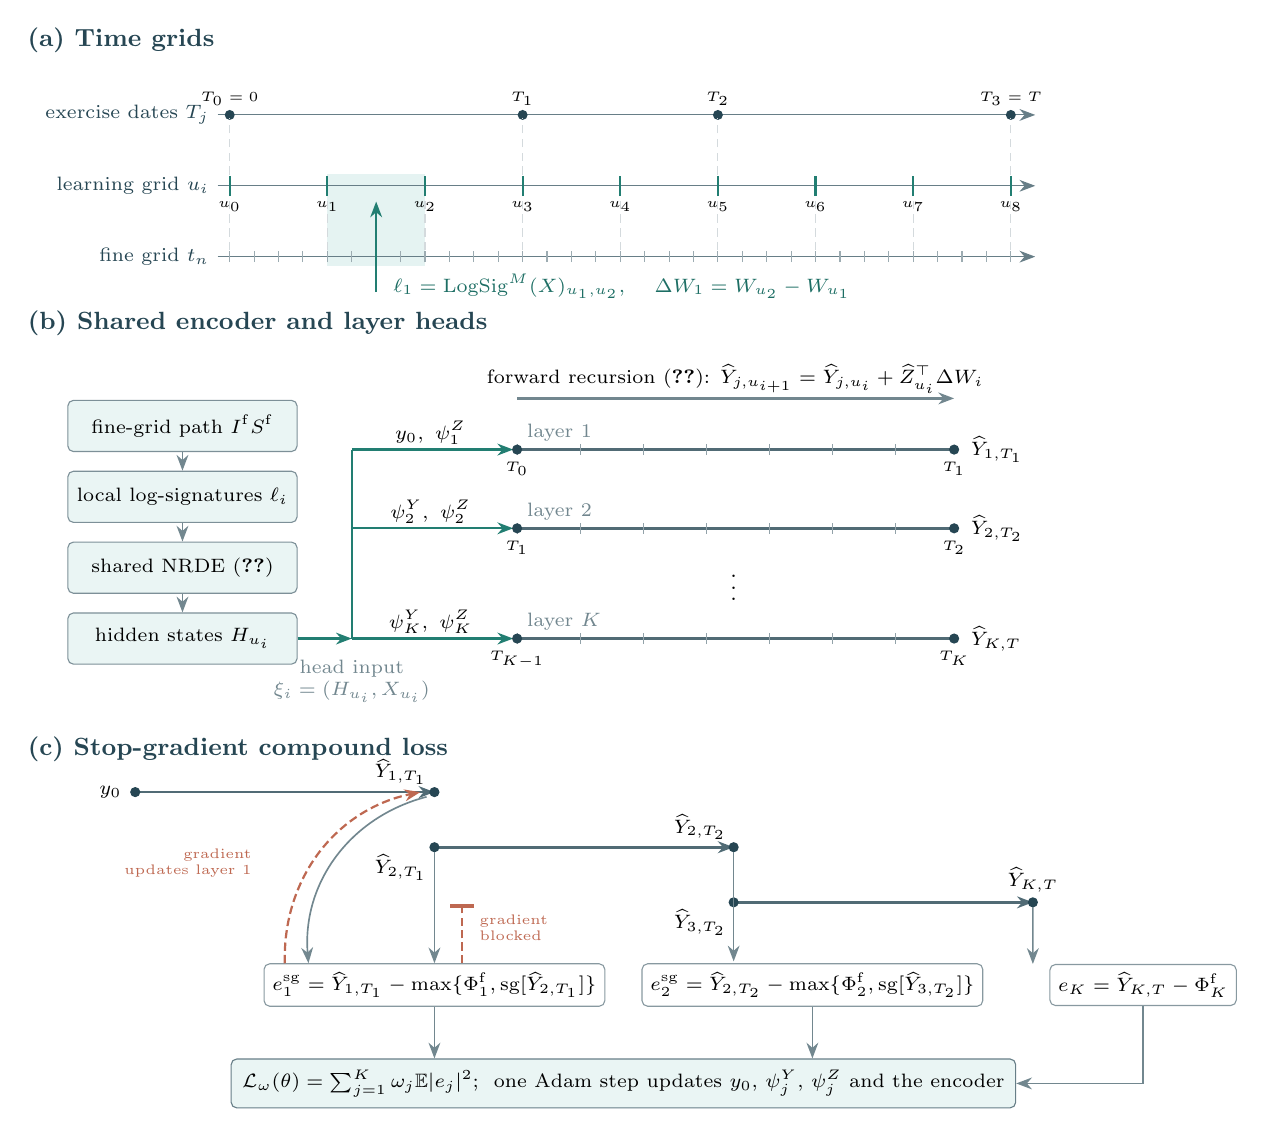
\begin{tikzpicture}[
  font=\footnotesize,
  >={Stealth[length=2mm]},
  plab/.style={font=\small\bfseries, text=cInk, anchor=west, inner sep=0pt},
  rowlab/.style={font=\scriptsize, text=cInk, anchor=east, inner sep=2pt},
  note/.style={font=\scriptsize, text=cInk!65},
  ebox/.style={draw=cInk!60, fill=cStop!10, rounded corners=2pt, align=center,
               inner sep=3pt, minimum height=6.5mm, text width=2.7cm, font=\scriptsize},
  ar/.style={->, draw=cInk!65, line width=0.6pt},
  hd/.style={->, draw=cStop!80!black, line width=0.8pt},
  lay/.style={draw=cInk!80, line width=1pt},
  dotn/.style={circle, fill=cInk, inner sep=1.3pt},
  rbox/.style={draw=cInk!55, fill=white, rounded corners=2pt, align=center,
               inner sep=3pt, font=\scriptsize},
  lbox/.style={draw=cInk!70, fill=cStop!10, rounded corners=2pt, align=center,
               inner sep=4pt, font=\scriptsize},
  grad/.style={->, draw=cJoint!85!black, line width=0.8pt, dash pattern=on 3pt off 1.5pt},
  gstop/.style={draw=cJoint!85!black, line width=0.8pt, dash pattern=on 3pt off 1.5pt,
                -{Bar[width=3mm,line width=1.4pt]}},
]

%======================================================================
% (a) Time grids
%======================================================================
\begin{scope}[shift={(0,0)}, x=0.31cm]
  \node[plab] at (-8.3,2.75) {(a) Time grids};
  \fill[cStop!12] (4,-0.12) rectangle (8,1.05);
  % fine grid
  \draw[->, cInk!70] (-0.5,0) -- (33,0);
  \foreach \n in {0,...,32}{\draw[cInk!45] (\n,-0.07) -- (\n,0.07);}
  \node[rowlab] at (-0.6,0) {fine grid $t_n$};
  % learning grid
  \draw[->, cInk!70] (-0.5,0.9) -- (33,0.9);
  \foreach \n in {0,4,...,32}{\draw[thick, cStop!80!black] (\n,0.77) -- (\n,1.03);}
  \foreach \n/\l in {0/0,4/1,8/2,12/3,16/4,20/5,24/6,28/7,32/8}{
    \node[font=\tiny, anchor=north, inner sep=1.5pt] at (\n,0.76) {$u_{\l}$};}
  \node[rowlab] at (-0.6,0.9) {learning grid $u_i$};
  % exercise dates
  \draw[->, cInk!70] (-0.5,1.8) -- (33,1.8);
  \foreach \n in {0,12,20,32}{\fill[cInk] (\n,1.8) circle (1.8pt);}
  \foreach \n/\l in {0/{T_0=0},12/{T_1},20/{T_2},32/{T_3=T}}{
    \node[font=\tiny, anchor=south, inner sep=2pt] at (\n,1.84) {$\l$};}
  \node[rowlab] at (-0.6,1.8) {exercise dates $T_j$};
  \foreach \n in {0,4,...,32}{\draw[densely dashed, cInk!20] (\n,0.08) -- (\n,0.76);}
  \foreach \n in {0,12,20,32}{\draw[densely dashed, cInk!20] (\n,1.04) -- (\n,1.76);}
  % one learning interval
  \draw[->, cStop!80!black, thick] (6,-0.45) -- (6,0.7);
  \node[note, anchor=west, text=cStop!70!black] at (6.3,-0.38)
    {$\ell_1=\LogSig^M(X)_{u_1,u_2}$, \quad $\Delta W_1=W_{u_2}-W_{u_1}$};
\end{scope}

%======================================================================
% (b) Shared encoder and layer heads
%======================================================================
\begin{scope}[shift={(0,-1.6)}]
  \node[plab] at (-2.57,0.75) {(b) Shared encoder and layer heads};
  \node[ebox] (E1) at (-0.6,-0.55) {fine-grid path $\Ipl S^{\mathrm f}$};
  \node[ebox] (E2) at (-0.6,-1.45) {local log-signatures $\ell_i$};
  \node[ebox] (E3) at (-0.6,-2.35) {shared NRDE \eqref{eq:logode}};
  \node[ebox] (E4) at (-0.6,-3.25) {hidden states $H_{u_i}$};
  \draw[ar] (E1) -- (E2); \draw[ar] (E2) -- (E3); \draw[ar] (E3) -- (E4);
  % heads bus
  \draw[cStop!80!black, line width=0.8pt] (1.55,-0.85) -- (1.55,-3.25);
  \draw[hd] (E4.east) -- (1.55,-3.25);
  \node[note, anchor=north, align=center] at (1.55,-3.4) {head input\\ $\xi_i=(H_{u_i},X_{u_i})$};
  % layers
  \foreach \y/\lab/\hl/\ta/\tb/\val in {%
     -0.85/{layer 1}/{y_0,\ \psi^Z_1}/{T_0}/{T_1}/{\hY_{1,T_1}},
     -1.85/{layer 2}/{\psi^Y_2,\ \psi^Z_2}/{T_1}/{T_2}/{\hY_{2,T_2}},
     -3.25/{layer $K$}/{\psi^Y_K,\ \psi^Z_K}/{T_{K-1}}/{T_K}/{\hY_{K,T}}}{
    \draw[hd] (1.55,\y) -- (3.6,\y);
    \node[font=\scriptsize, anchor=south, inner sep=1.5pt] at (2.55,\y) {$\hl$};
    \draw[lay] (3.65,\y) -- (9.2,\y);
    \foreach \x in {3.65,4.45,...,9.2}{\draw[cInk!50] (\x,\y-0.07) -- (\x,\y+0.07);}
    \node[dotn] at (3.65,\y) {}; \node[dotn] at (9.2,\y) {};
    \node[note, anchor=south west, inner sep=2pt] at (3.7,\y+0.03) {\lab};
    \node[font=\tiny, anchor=north, inner sep=2pt] at (3.65,\y-0.08) {$\ta$};
    \node[font=\tiny, anchor=north, inner sep=2pt] at (9.2,\y-0.08) {$\tb$};
    \node[font=\scriptsize, anchor=west, inner sep=3pt] at (9.3,\y) {$\val$};}
  \node at (6.4,-2.5) {$\vdots$};
  \draw[->, cInk!65, line width=0.8pt] (3.65,-0.2) -- (9.2,-0.2);
  \node[font=\scriptsize, anchor=south, inner sep=1.5pt] at (6.42,-0.2)
    {forward recursion \eqref{eq:scheme}: $\hY_{j,u_{i+1}}=\hY_{j,u_i}+\hZ_{u_i}^\top\Delta W_i$};
\end{scope}

%======================================================================
% (c) Stop-gradient compound loss
%======================================================================
\begin{scope}[shift={(0,-6.5)}]
  \node[plab] at (-2.57,0.25) {(c) Stop-gradient compound loss};
  % staircase of layers
  \draw[lay, ->] (-1.2,-0.3) -- (2.6,-0.3);
  \draw[lay, ->] (2.6,-1.0) -- (6.4,-1.0);
  \draw[lay, ->] (6.4,-1.7) -- (10.2,-1.7);
  \foreach \p in {(-1.2,-0.3),(2.6,-0.3),(2.6,-1.0),(6.4,-1.0),(6.4,-1.7),(10.2,-1.7)}{\node[dotn] at \p {};}
  \node[font=\scriptsize, anchor=east] at (-1.25,-0.3) {$y_0$};
  \node[font=\scriptsize, anchor=south east, inner sep=1pt] at (2.55,-0.25) {$\hY_{1,T_1}$};
  \node[font=\scriptsize, anchor=south east, inner sep=1pt] at (6.35,-0.95) {$\hY_{2,T_2}$};
  \node[font=\scriptsize, anchor=south, inner sep=2pt] at (10.2,-1.65) {$\hY_{K,T}$};
  \node[font=\scriptsize, anchor=north east, inner sep=1pt] at (2.55,-1.05) {$\hY_{2,T_1}$};
  \node[font=\scriptsize, anchor=north east, inner sep=1pt] at (6.35,-1.75) {$\hY_{3,T_2}$};
  % residual boxes
  \node[rbox] (e1) at (2.6,-2.75) {$e^{\sg}_1=\hY_{1,T_1}-\max\{\Phi^{\mathrm f}_1,\sg[\hY_{2,T_1}]\}$};
  \node[rbox] (e2) at (7.4,-2.75) {$e^{\sg}_2=\hY_{2,T_2}-\max\{\Phi^{\mathrm f}_2,\sg[\hY_{3,T_2}]\}$};
  \node[rbox] (eK) at (11.6,-2.75) {$e_K=\hY_{K,T}-\Phi^{\mathrm f}_K$};
  % layer 1 end value: forward and gradient
  \draw[ar] (2.5,-0.36) to[bend right=40] ($(e1.north)+(-1.6,0)$);
  \draw[grad] ($(e1.north)+(-1.9,0)$) to[bend left=40] (2.42,-0.3);
  \node[font=\tiny, text=cJoint!85!black, anchor=east, align=right] at (0.4,-1.2) {gradient\\ updates layer 1};
  % continuation value: forward, gradient blocked
  \draw[ar] (2.6,-1.06) -- ($(e1.north)+(0,0)$);
  \draw[gstop] ($(e1.north)+(0.35,0)$) -- ++(0,0.75);
  \node[font=\tiny, text=cJoint!85!black, anchor=west, align=left] at ($(e1.north)+(0.45,0.45)$) {gradient\\ blocked};
  \draw[ar] (6.4,-1.06) -- (6.4,-2.45);
  \draw[ar] (10.2,-1.76) -- ($(eK.north)+(-1.4,0)$);
  % loss
  \node[lbox] (L) at (5.0,-4.0) {$\cL_\omega(\theta)=\sum_{j=1}^K\omega_j\E\abs{e_j}^2$; \ one Adam step updates $y_0$, $\psi^Y_j$, $\psi^Z_j$ and the encoder};
  \draw[ar] (e1.south) -- (e1.south |- L.north);
  \draw[ar] (e2.south) -- (e2.south |- L.north);
  \draw[ar] (eK.south) |- (L.east);
\end{scope}
\end{tikzpicture}
}
\caption{Overview of the method: (a) time grids, (b) shared encoder and layer heads, (c) stop-gradient compound loss.}
\label{fig:framework}
\end{figure}

\subsection{Grids and local log-signatures}\label{sec:grids}

We use two nested time grids: a fine grid $t_n=n\hf$, on which asset paths are simulated and payoffs are monitored, and a coarser learning grid $u_i=ih$ with $h=T/N$, on which the encoder and the BSDE recursion operate. The learning grid contains every exercise date, and the refinement ratio $m=h/\hf$ is an integer. The simulated prices $S^{\mathrm f}_{t_n}$ are driven by the increments of $W$ on the fine grid, exactly for geometric Brownian motion and by the Euler scheme otherwise, and $\Ipl S^{\mathrm f}$ denotes their piecewise-linear interpolation. Accordingly, the monitored payoffs and links are given by
\[
\Phi^{\mathrm f}_j=\Phi_j\left(\Ipl S^{\mathrm f}|_{[0,T_j]}\right),\quad g^{\mathrm f}_j(y)=g_j\left(\Ipl S^{\mathrm f}|_{[0,T_j]},y\right).
\]

The encoder takes as input the normalized time-augmented path $X_t=\left(t/T,\,D^{-1}(\Ipl S^{\mathrm f}_t-\mu)\right)\in\R^{1+d}$. The constants $\mu\in\R^d$ and the diagonal matrix $D$ are estimated once on a pilot sample and then frozen. The signature of $X$ on $[s,t]$ truncated at level $M$ collects the iterated integrals
\[
\Sig^{M}(X)_{s,t}=\left(1,\ \int_{s<v<t}\dd X_{v},\ \int_{s<v_1<v_2<t}\dd X_{v_1}\otimes\dd X_{v_2},\ \dots\right)
\]
up to order $M$. Chen's identity $\Sig^M(X)_{0,t}=\Sig^M(X)_{0,s}\otimes\Sig^M(X)_{s,t}$ assembles the signature of the whole path from those of its pieces \cite{lyons1998}. The log-signature $\LogSig^M=\log_\otimes\Sig^M$ encodes the same information in $q_M$ coordinates, far fewer than the signature. The encoder uses the local log-signatures
\begin{equation}\label{eq:local-logsig}
\ell_i=\LogSig^M(X)_{u_i,u_{i+1}}\in\R^{q_M},\quad i=0,\dots,N-1 .
\end{equation}
The first level records the increments of time and price, while the second level captures the signed L\'evy areas between coordinates. Since the L\'evy area between price coordinate $a$ and normalized time differs from $T^{-1}\int_{u_i}^{u_{i+1}}(X^a_t-X^a_{u_i})\dd t$ only by a multiple of the price increment, the level-two log-signature already encodes the local running integral of the price; \cref{lem:information} makes this precise.

\subsection{Shared Neural RDE encoder}\label{sec:encoder}

The hidden state $H_t\in\R^p$ starts from $H_0=\rho_\theta(X_0)$ and follows the log-ODE
\begin{equation}\label{eq:logode}
\frac{\dd H_s}{\dd s}=G_\theta(H_s)\,\frac{\ell_i}{h},\quad s\in[u_i,u_{i+1}],
\end{equation}
where $G_\theta:\R^p\to\R^{p\times q_M}$ is a neural vector field \cite{morrill2021}. A fixed number of Runge--Kutta sub-steps defines the update map $H_{u_{i+1}}=R_\theta(H_{u_i},\ell_i)$. A single state sequence $(H_{u_i})_{i\le N}$ extends across all layers without being reset at the exercise dates, and the encoder parameters are shared by every layer.

\subsection{Heads and forward recursion}\label{sec:heads}

Let $\xi_i=(H_{u_i},X_{u_i})$ denote the input of the heads at $u_i$, which contains the hidden state, the normalized price, and the time. The price at time zero is a trainable scalar $y_0$. For $j\ge2$, a value head outputs the initial value of layer $j$, and on every layer a hedge head outputs the integrand:
\[
\hY_{j,T_{j-1}}=\psi^Y_{j}(\xi_{i}),\quad u_i=T_{j-1},\quad
\hZ_{u_i}=\psi^Z_{j}(\xi_i),\quad u_i\in[T_{j-1},T_j).
\]
Within each layer, the value follows the forward Euler recursion
\begin{equation}\label{eq:scheme}
\hY_{1,0}=y_0,\quad \hY_{j,u_{i+1}}=\hY_{j,u_i}+\hZ_{u_i}^\top\Delta W_i,\quad u_i\in[T_{j-1},T_j),
\end{equation}
where $\Delta W_i=W_{u_{i+1}}-W_{u_i}$. Between grid points, we set $\hY_{j,t}=\hY_{j,T_{j-1}}+\int_{T_{j-1}}^t\hZ_s^\top\dd W_s$ with $\hZ$ piecewise constant. In the implementation, undiscounted values follow the step $(1+rh)\hY_{j,u_i}+\hZ_{u_i}^\top\Delta W_i$, and \cref{lem:discount} shows that the discrete discount factor $(1+rh)^{-i}$ maps this step exactly onto \eqref{eq:scheme}. The interface and terminal residuals are defined by
\begin{equation}\label{eq:residual}
e_j=\hY_{j,T_j}-g^{\mathrm f}_j\left(\hY_{j+1,T_j}\right),\quad j<K,\quad e_K=\hY_{K,T}-\Phi^{\mathrm f}_K .
\end{equation}

By construction, the network is non-anticipative. To make this precise, let $\cG^{\pi}_{u_i}=\sigma(S^{\mathrm f}_{t_n}:t_n\le u_i)$ denote the fine-grid filtration and $\cG^{M}_{u_i}=\sigma(\ell_0,\dots,\ell_{i-1})$ the encoder filtration.

\begin{lemma}[non-anticipation]\label{lem:nonanticipation}
For every parameter $\theta$, every level $M$, and every number of Runge--Kutta sub-steps:
\begin{enumerate}[label=(\roman*)]
\item $H_{u_i}$ is $\cG^{M}_{u_i}$-measurable and $\cG^{M}_{u_i}\subseteq\cG^{\pi}_{u_i}\subseteq\cF_{u_i}$;
\item $\hZ_{u_i}$ is $\cG^{M}_{u_i}$-measurable and $\hY_{j,T_{j-1}}$ is $\cG^{M}_{T_{j-1}}$-measurable;
\item if $\E\abs{\hY_{j,T_{j-1}}}^2+h\sum_{u_i\in[T_{j-1},T_j)}\E\abs{\hZ_{u_i}}^2<\infty$, then $t\mapsto\hY_{j,t}$ is a square-integrable martingale on $[T_{j-1},T_j]$.
\end{enumerate}
\end{lemma}

\begin{proof}[Proof sketch]
Each $\ell_k$ is a Borel function of the fine-grid prices on $[u_k,u_{k+1}]$, and $H_{u_{i+1}}$ is a Borel function of $(H_{u_i},\ell_i)$, so induction over $i$ yields (i). Part (ii) follows because the normalized price $X_{u_i}$ is determined by the level-one increments $\ell_0,\dots,\ell_{i-1}$. Part (iii) is a consequence of $\E[\Delta W_i\mid\cF_{u_i}]=0$ and It\^o's isometry. See \cref{app:nonanticipation}.
\end{proof}

\begin{remark}\label{rem:nonanticipation}
The network value is a martingale on every layer for every choice of parameters, trained or not, and this is the only property of the architecture used in \cref{sec:analysis}. The lemma dictates two design rules: the hedge head at $u_i$ must not access the current increment $\ell_i$, and the normalization statistics $(\mu,D)$ must not be computed on the active training batch. Violating either rule induces a look-ahead bias with $\E[\hZ_{u_i}^\top\Delta W_i]\ne0$, which invalidates both the a posteriori estimate and the dual upper bound.
\end{remark}

\subsection{Stop-gradient interface targets}\label{sec:loss}

The training objective is the weighted endpoint loss
\begin{equation}\label{eq:loss}
\cL_\omega(\theta)=\sum_{j=1}^K\omega_j\,\E\abs{e_j}^2,\quad \omega_j>0,
\end{equation}
which is estimated on fresh batches of simulated paths. We write $\cL(\theta)$ for the unweighted loss with $\omega_j=1$; the experiments use $\omega_j=1/K$. The residual $e_j$ depends on the parameters through both sides of the interface: the left side $\hY_{j,T_j}$ depends on the heads of layer $j$ and on the encoder, whereas the target $g^{\mathrm f}_j(\hY_{j+1,T_j})$ depends on the value head of layer $j+1$. \emph{Joint training} \cite{huang2026} differentiates both sides.

\emph{Stop-gradient training} detaches the target instead. Denoting by $\sg[\cdot]$ the stop-gradient operator, which acts as the identity in the forward pass but has zero derivative in the backward pass, we define the detached residual
\begin{equation}\label{eq:sg-residual}
e^{\sg}_j=\hY_{j,T_j}-g^{\mathrm f}_j\left(\sg[\hY_{j+1,T_j}]\right).
\end{equation}
Write $\cL^{\sg}_\omega$ for \eqref{eq:loss} with $e^{\sg}_j$ in place of $e_j$. The case $K=2$ with the Bermudan link shows the difference. Let $\theta^Y_2$ denote the parameters of the value head $\psi^Y_2$, and write $v=\hY_{2,T_1}$ for its output. The value $v$ enters both residuals: as the initial value of layer $2$ in $e_2=v+\sum_{u_i\in[T_1,T)}\hZ_{u_i}^\top\Delta W_i-\Phi^{\mathrm f}_2$, and as the continuation value in $e_1=\hY_{1,T_1}-\max\{\Phi^{\mathrm f}_1,v\}$. By the chain rule,
\begin{equation}\label{eq:grad-K2}
\begin{aligned}
\nabla_{\theta^Y_2}\cL_\omega&=2\,\E\Bigl[\bigl(\omega_2e_2-\omega_1e_1\1\{v>\Phi^{\mathrm f}_1\}\bigr)\nabla_{\theta^Y_2}v\Bigr] &&\text{(joint)},\\
\nabla_{\theta^Y_2}\cL^{\sg}_\omega&=2\,\E\bigl[\omega_2e_2\,\nabla_{\theta^Y_2}v\bigr] &&\text{(stop-gradient)}.
\end{aligned}
\end{equation}
So the value head $\psi^Y_2$ is updated using only the second-layer residual $e_2$. Now suppose that the value head permits local perturbations $v+\varepsilon h$ for every bounded $\cG^M_{T_1}$-measurable function $h$, changing the residual to $e_2+\varepsilon h$. At a stationary point, $0=\left.\frac{\dd}{\dd\varepsilon}\omega_2\E[(e_2+\varepsilon h)^2]\right|_{\varepsilon=0}=2\omega_2\E[e_2h]$. Because this equality holds for every such $h$, it implies $\E[e_2\mid\cG^M_{T_1}]=0$. Hence, by the martingale property of layer $2$ (\cref{lem:nonanticipation}(iii)), we have $v=\E[\Phi^{\mathrm f}_2\mid\cG^M_{T_1}]$. However, under joint training, we have
\[
v-\E[\Phi^{\mathrm f}_2\mid\cG^M_{T_1}]=\frac{\omega_1}{\omega_2}\E\left[e_1\1\{v>\Phi^{\mathrm f}_1\}\bigm|\cG^M_{T_1}\right].
\]
Thus, the first-layer residual can shift $v$ away from the
conditional expectation of the future payoff. On paths where
$v>\Phi^{\mathrm f}_1$, the residual is $e_1=\hY_{1,T_1}-v$. If $e_1>0$, the first-layer prediction exceeds $v$, so increasing $v$ reduces the first-layer squared residual locally. This will accumulate errors through layers. Stop-gradient training removes this contribution to the update of the second-layer value head.  \cref{thm:stationary} states this observation detailedly for general $K$.

This construction transfers the semi-gradient rule of temporal-difference learning and the target network of deep $Q$-learning \cite{sutton2018,mnih2015} to the compound BSDE. Two related variants appear in \cref{sec:experiments}. The exponential moving average (EMA) variant evaluates the target with a slowly updated moving average of the parameters, and layerwise training uses the same detached target but trains the layers one at a time, backward from $T$. \Cref{fig:interface} compares the gradient paths.

\begin{figure}[htbp]
\centering
\resizebox{\textwidth}{!}{% Interface training variants.  Top: the forward computation shared by all
% variants.  Bottom: where the gradient of |e_j|^2 goes in each variant.
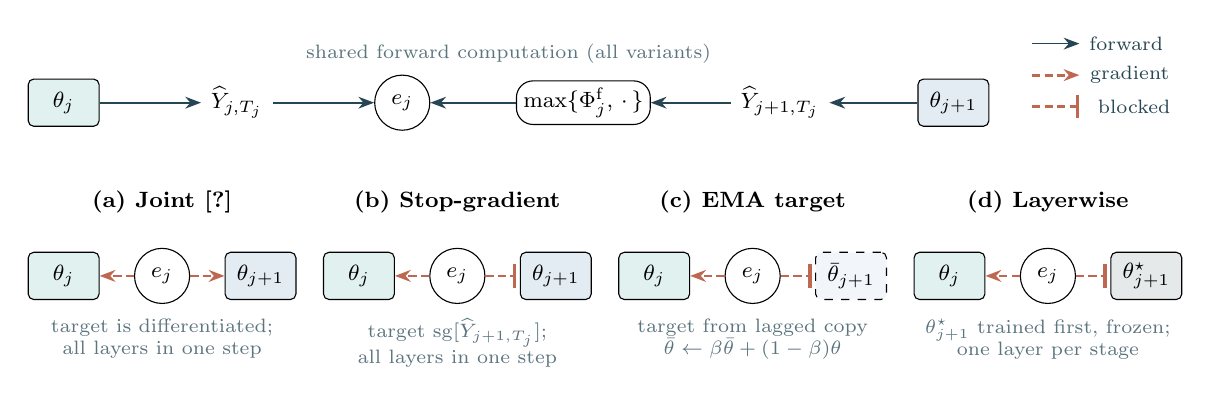
\begin{tikzpicture}[
    font=\footnotesize,
    >={Stealth[length=2mm]},
    param/.style={draw, rounded corners=2pt, minimum width=9mm, minimum height=6mm, inner sep=2pt},
    pj/.style={param, fill=cStop!14},
    pn/.style={param, fill=cFull!22},
    pema/.style={param, fill=cFull!10, dashed},
    pfrozen/.style={param, fill=cInk!12},
    res/.style={draw, circle, fill=white, inner sep=1pt, minimum size=7mm},
    tgt/.style={draw, rounded corners=6pt, fill=white, inner sep=2.5pt},
    f/.style={->, cInk, line width=0.6pt},
    g/.style={->, cJoint!85!black, line width=1pt, dash pattern=on 3pt off 1.5pt},
    gstop/.style={cJoint!85!black, line width=1pt, dash pattern=on 3pt off 1.5pt,
                  -{Bar[width=3mm,line width=1.4pt]}},
    ttl/.style={font=\footnotesize\bfseries, anchor=south, inner sep=1pt},
    nt/.style={font=\scriptsize, text=cInk!75, anchor=north, align=center, inner sep=1pt},
  ]

% ---------------- shared forward computation ----------------
\node[pj]  (thj) at (0,0)    {$\theta_j$};
\node      (yj)  at (2.2,0)  {$\hY_{j,T_j}$};
\node[res] (e)   at (4.3,0)  {$e_j$};
\node[tgt] (mx)  at (6.6,0)  {$\max\{\Phi^{\mathrm f}_j,\,\cdot\,\}$};
\node      (yn)  at (9.1,0)  {$\hY_{j+1,T_j}$};
\node[pn]  (thn) at (11.3,0) {$\theta_{j+1}$};
\draw[f] (thj) -- (yj); \draw[f] (yj) -- (e); \draw[f] (mx) -- (e);
\draw[f] (yn) -- (mx); \draw[f] (thn) -- (yn);
\node[font=\scriptsize, text=cInk!75, anchor=south] at (5.65,0.38)
  {shared forward computation (all variants)};
\draw[f] (12.3,0.75) -- ++(0.6,0) node[right, font=\scriptsize, text=cInk] {forward};
\draw[g] (12.3,0.35) -- ++(0.6,0) node[right, font=\scriptsize, text=cInk] {gradient};
\draw[gstop] (12.3,-0.05) -- ++(0.6,0) node[right, font=\scriptsize, text=cInk, xshift=1mm] {blocked};

% ---------------- the four gradient patterns ----------------
\foreach \x/\ttl in {0/{(a) Joint \cite{huang2026}}, 3.75/{(b) Stop-gradient}, 7.5/{(c) EMA target}, 11.25/{(d) Layerwise}}{
  \node[ttl] at (\x+1.25,-1.45) {\ttl};
}
% (a) joint
\begin{scope}[shift={(0,-2.2)}]
  \node[pj] (a1) at (0,0) {$\theta_j$}; \node[res] (a2) at (1.25,0) {$e_j$}; \node[pn] (a3) at (2.5,0) {$\theta_{j+1}$};
  \draw[g] (a2) -- (a1); \draw[g] (a2) -- (a3);
  \node[nt] at (1.25,-0.5) {target is differentiated;\\ all layers in one step};
\end{scope}
% (b) stop-gradient
\begin{scope}[shift={(3.75,-2.2)}]
  \node[pj] (b1) at (0,0) {$\theta_j$}; \node[res] (b2) at (1.25,0) {$e_j$}; \node[pn] (b3) at (2.5,0) {$\theta_{j+1}$};
  \draw[g] (b2) -- (b1); \draw[gstop] (b2) -- ($(b2)!0.6!(b3)$);
  \node[nt] at (1.25,-0.5) {target $\sg[\hY_{j+1,T_j}]$;\\ all layers in one step};
\end{scope}
% (c) EMA target
\begin{scope}[shift={(7.5,-2.2)}]
  \node[pj] (c1) at (0,0) {$\theta_j$}; \node[res] (c2) at (1.25,0) {$e_j$}; \node[pema] (c3) at (2.5,0) {$\bar\theta_{j+1}$};
  \draw[g] (c2) -- (c1); \draw[gstop] (c2) -- ($(c2)!0.6!(c3)$);
  \node[nt] at (1.25,-0.5) {target from lagged copy\\ $\bar\theta\leftarrow\beta\bar\theta+(1-\beta)\theta$};
\end{scope}
% (d) layerwise
\begin{scope}[shift={(11.25,-2.2)}]
  \node[pj] (d1) at (0,0) {$\theta_j$}; \node[res] (d2) at (1.25,0) {$e_j$}; \node[pfrozen] (d3) at (2.5,0) {$\theta^\star_{j+1}$};
  \draw[g] (d2) -- (d1); \draw[gstop] (d2) -- ($(d2)!0.6!(d3)$);
  \node[nt] at (1.25,-0.5) {$\theta^\star_{j+1}$ trained first, frozen;\\ one layer per stage};
\end{scope}
\end{tikzpicture}
}
\caption{Interface training variants. Top: forward computation. Bottom: gradient of $|e_j|^2$.}
\label{fig:interface}
\end{figure}

\begin{algorithm}[htbp]
\caption{Stop-gradient training of the log-signature compound BSDE}
\label{alg:train}
\begin{algorithmic}[1]
\Require grids $(t_n)$, $(u_i)\ni T_j$; level $M$; weights $\omega_j$; batch size $B$; number of updates $n_{\mathrm{it}}$
\For{$n=1,\dots,n_{\mathrm{it}}$}
  \State simulate $B$ fine-grid paths $S^{\mathrm f}$ with increments $\Delta W$
  \State compute $\ell_i$ by \eqref{eq:local-logsig} and $H_{u_{i+1}}=R_\theta(H_{u_i},\ell_i)$ for $i<N$
  \For{$j=1,\dots,K$}
    \State $\hY_{j,T_{j-1}}\gets y_0$ if $j=1$, else $\psi^Y_j(\xi_i)$ with $u_i=T_{j-1}$
    \State run \eqref{eq:scheme} on $[T_{j-1},T_j]$ with $\hZ_{u_i}=\psi^Z_j(\xi_i)$
  \EndFor
  \State form $e^{\sg}_j$ by \eqref{eq:sg-residual} and the batch loss $\frac1B\sum_b\sum_j\omega_j\abs{e^{\sg,(b)}_j}^2$
  \State update all parameters $\theta$ by one Adam step
\EndFor
\end{algorithmic}
\end{algorithm}

\subsection{Exercise rule and primal--dual bounds}\label{sec:certificates}

A trained network defines both an exercise rule and a dual martingale. Given a margin $\eex\ge0$, the rule exercises at the first date at which the payoff is positive and exceeds the predicted continuation value by at least $\eex$:
\[
\hat\tau=\min\bigl\{T_k,\ k<K:\ \Phi^{\mathrm f}_k>0,\ \Phi^{\mathrm f}_k\ge\hY_{k+1,T_k}+\eex\bigr\}\wedge T_K .
\]
The hedge heads define the martingale $\int_0^t\hZ_s^\top\dd W_s$, accumulated across all layers, and the lower and upper bounds are
\begin{equation}\label{eq:bounds}
L_0=\E\,\Phi^{\mathrm f}_{\hat\tau},\quad
U_0=\E\max_{1\le k\le K}\left(\Phi^{\mathrm f}_k-\int_0^{T_k}\hZ_s^\top\dd W_s\right),
\end{equation}
following the primal--dual construction of \cite{rogers2002,haugh2004}. Both bounds are estimated on independent test paths in a single forward pass. The asset position is recovered from $\hZ$ by $\hat\Delta_{u_i}=(\sigma(u_i,S_{u_i})^\top)^{-1}\hZ_{u_i}$ when $\sigma$ has full rank.

%======================================================================
\seeftion{Error analysis}\label{sec:analysis}
%======================================================================

The total error of a trained network stems from four sources: monitoring the payoffs on the fine grid, holding the hedge constant over each learning step, truncating the log-signature at level $M$, and approximating the optimal measurable outputs with a finite-capacity network. \Cref{sec:disc,sec:aposteriori} control the first two sources and relate the loss to the error. \Cref{sec:info} incorporates truncation and assembles the error budget. \Cref{sec:stationary} then compares the stationary points of the two interface rules, and \cref{sec:certificate} turns the trained network into price bounds. Throughout, \cref{ass:sde,ass:link} hold, all quantities are discounted, and $C$ denotes a constant depending only on $T$, $L_g$, $b$, and $\sigma$, but never on $K$, $h$, $\hf$, $M$, or $\theta$.

The network targets the \emph{monitored solution} $(Y^{\mathrm f}_j,Z^{\mathrm f}_j)$, namely the solution of \eqref{eq:cbsde} with links $g^{\mathrm f}_j$, and its price $V^{\mathrm f}_0=Y^{\mathrm f}_{1,0}$. For a process $Z$, let
\[
\bZ_{u_i}=\frac1h\,\E\left[\int_{u_i}^{u_{i+1}}Z_t\dd t\Bigm|\cF_{u_i}\right],\quad
\varepsilon^\pi(Z)=\sum_{i}\E\int_{u_i}^{u_{i+1}}\abs{Z_t-\bZ_{u_i}}^2\dd t,
\]
where $Z=Z_j$ on $[T_{j-1},T_j)$. The integrand $\bZ_{u_i}$ is the best $\cF_{u_i}$-measurable constant approximation of $Z$ on $[u_i,u_{i+1})$ in $L^2$, and $\varepsilon^\pi(Z)$ is the error of the best hedge that is rebalanced only on the learning grid. The monitoring error is $\emon=\E\norm{S-\Ipl S^{\mathrm f}}_T^2$.

\subsection{Discretization}\label{sec:disc}

\begin{theorem}[discretization]\label{thm:discretisation}
\leavevmode
\begin{enumerate}[label=(\alph*)]
\item $\max_j\sup_{t}\E\abs{Y_{j,t}-Y^{\mathrm f}_{j,t}}^2\le L_g^2\emon$ and $\sum_{j=1}^K\E\int_{T_{j-1}}^{T_j}\abs{Z_{j,t}-Z^{\mathrm f}_{j,t}}^2\dd t\le KL_g^2\emon$.
\item $\emon\le C\hf\log(2T/\hf)$ and $\varepsilon^\pi(Z)\le CKh$.
\end{enumerate}
\end{theorem}

\begin{proof}[Proof sketch]
For (a), backward induction over the layers and the max form of \cref{ass:link} yield $\abs{Y_{j,t}-Y^{\mathrm f}_{j,t}}\le L_g\E[\norm{S-\Ipl S^{\mathrm f}}_T\mid\cF_t]$, and It\^o's isometry on each layer bounds the hedge difference by the terminal difference. For (b), the Euler sup-norm estimate of \cite[Thm.~4.2]{zhang2004} transfers to the interpolation $\Ipl S^{\mathrm f}$ with a factor of $9$. Moreover, the layer terminal value $g_j(S,u_{j+1}(T_j,S))$ is Lipschitz in the path by \cref{thm:wellposed}(iii), so Zhang's $L^2$-regularity theorem \cite{zhang2004}, applied to smooth approximations of each layer, gives $\varepsilon^\pi(Z_j)\le Ch$ per layer. See \cref{app:discretisation}.
\end{proof}

\begin{remark}\label{rem:discretisation}
Monitoring changes the price and the hedge by $O(\sqrt{\hf\log(1/\hf)})$, uniformly in $K$. Rebalancing on the learning grid incurs an error of $O(Kh)$, or $O(T/n)$ with $n$ learning steps per layer; consequently, the irreducible discretization floor is governed by the number of learning steps per layer. The factor $K$ reflects the kink that each interface creates in the layer payoff, and \cref{fig:floor}(c) confirms this scaling. For a single BSDE, Zhang \cite{zhang2004} obtains $\varepsilon^\pi(Z)=O(h)$, and Bayraktar, Feng, and Zhang \cite{bayraktar2024} bound the error of their backward signature scheme in terms of the step size, the truncation order, and the network errors. Part (b) extends the regularity result to $K$ linked layers on path space.
\end{remark}

\subsection{A posteriori estimate}\label{sec:aposteriori}

\begin{theorem}[a posteriori estimate]\label{thm:aposteriori}
Let $y_0$, $\hY_{j,T_{j-1}}$, and $\hZ_{u_i}$ be any square-integrable outputs adapted to $\F$, in particular those of any network (\cref{lem:nonanticipation}). Then
\begin{equation}\label{eq:aposteriori}
\max_j\sup_{t}\E\abs{Y^{\mathrm f}_{j,t}-\hY_{j,t}}^2+\sum_{j=1}^K\E\int_{T_{j-1}}^{T_j}\abs{Z^{\mathrm f}_{j,t}-\hZ_t}^2\dd t\le2K\,\cL(\theta).
\end{equation}
Each of the two terms is bounded by $K\cL(\theta)$, and $\abs{y_0-V^{\mathrm f}_0}\le\sum_j\norm{e_j}_{L^2}$. Conversely, $\cL(\theta)\le4\sum_j\E\abs{Y^{\mathrm f}_{j,T_j}-\hY_{j,T_j}}^2$. With $(Y,Z)$ in place of $(Y^{\mathrm f},Z^{\mathrm f})$, the right-hand side of \eqref{eq:aposteriori} becomes $4K\cL(\theta)+2(K+1)L_g^2\emon$.
\end{theorem}

\begin{proof}[Proof sketch]
Set $\delta Y_j=Y^{\mathrm f}_j-\hY_j$. Since both processes are martingales on each layer, It\^o's isometry gives $\E\int\abs{\delta Z_j}^2=\norm{\delta Y_{j,T_j}}^2_{L^2}-\norm{\delta Y_{j,T_{j-1}}}^2_{L^2}$. As the link is $1$-Lipschitz in $y$, we have $\norm{\delta Y_{j,T_j}}_{L^2}\le\norm{\delta Y_{j+1,T_j}}_{L^2}+\norm{e_j}_{L^2}$, and iterating from $j=K$ yields $\norm{\delta Y_{j,T_j}}_{L^2}\le\sum_{k\ge j}\norm{e_k}_{L^2}$. Telescoping the isometries then gives the bound $(\sum_j\norm{e_j}_{L^2})^2\le K\cL$. See \cref{app:aposteriori}.
\end{proof}

\begin{remark}\label{rem:aposteriori}
Whereas the approximation error is unobservable, the training loss is directly computable; \cref{thm:aposteriori} bridges the two for any adapted network, regardless of how it is trained. The converse inequality shows that loss and error are equivalent up to a factor of $4K$, and this equivalence links training to accuracy in \cref{thm:attainable,thm:primaldual}. Huang and Oosterlee \cite[Thm.~3.4]{huang2026} prove an a posteriori bound for general drivers under the condition $6T^2K_y^2<1$, and Han and Long \cite{han2020convergence} prove a single-layer analogue for the deep BSDE method under a weak-coupling condition. By contrast, discounting makes our scheme an exact martingale transform, so only the $1$-Lipschitz property of the link in $y$ is needed, and no condition on $h$, on the driver, or on the Markov property remains.
\end{remark}

\subsection{Log-signature information and the error budget}\label{sec:info}

The next assumption requires the simulated price to be a Markov chain on the fine grid. It holds for the exact simulation of geometric Brownian motion and for the Euler scheme, but fails for rough volatility models.

\begin{assumption}\label{ass:obs}
$S^{\mathrm f}_{t_{n+1}}=\Psi_n(S^{\mathrm f}_{t_n},W_{t_{n+1}}-W_{t_n})$ for Borel maps $\Psi_n$, and $s_0$ is deterministic.
\end{assumption}

The truncation error quantifies the part of the targets that is lost by conditioning on the encoder filtration $\cG^M$ instead of the fine-grid filtration:
\[
\etr(M)=\sum_{j=2}^K\E\bigl\lvert Y^{\mathrm f}_{j,T_{j-1}}-\E[Y^{\mathrm f}_{j,T_{j-1}}\mid\cG^{M}_{T_{j-1}}]\bigr\rvert^2+h\sum_i\E\bigl\lvert\bZ^{\mathrm f}_{u_i}-\E[\bZ^{\mathrm f}_{u_i}\mid\cG^{M}_{u_i}]\bigr\rvert^2 .
\]

\begin{lemma}[information]\label{lem:information}
Let \cref{ass:obs} hold.
\begin{enumerate}[label=(\roman*)]
\item $Y^{\mathrm f}_{j,u_i}$ and $\bZ^{\mathrm f}_{u_i}$ are $\cG^{\pi}_{u_i}$-measurable for $u_i\in[T_{j-1},T_j)$.
\item $\cG^{M}_{u_i}\subseteq\cG^{M+1}_{u_i}$, so $\etr(M)$ is nonincreasing in $M$.
\item If $M\ge m$, then $\cG^{M}_{u_i}=\cG^{\pi}_{u_i}$ for all $i$ and $\etr(M)=0$.
\item If every $\Phi_j$ depends on the current price only, then $\etr(M)=0$ for $M\ge1$. If every $\Phi_j$ depends on the current price and $\int_0^{T_j}\Ipl S^{\mathrm f}_t\dd t$ only, as for arithmetic Asian and Amerasian payoffs, then $\etr(M)=0$ for all $M\ge2$, regardless of $m$.
\end{enumerate}
\end{lemma}

\begin{proof}[Proof sketch]
Under \cref{ass:obs}, future prices depend on the past only through the grid prices, which proves (i), and part (ii) follows from the tower property. For (iii), the coordinates of $\ell_i$ with $r$ time letters followed by one price letter are linear combinations of the $m$ fine increments on $[u_i,u_{i+1}]$, and the coefficient matrix is of Vandermonde type with determinant $(\hf/T)^{m(m-1)/2}>0$. For (iv), the first level determines the current price and the second level the running integral, and this pair is a Markov state for the corresponding payoffs. See \cref{app:information}.
\end{proof}

\begin{remark}\label{rem:information}
The lemma provides a rule for choosing the truncation level: current-price payoffs require $M=1$, average-type payoffs require $M=2$, and level $m$ recovers the entire monitored path. Refining the learning grid lowers $m$ and hence the level needed for exact recovery. Universal approximation results for signatures \cite{lyons1998,cuchiero2025} guarantee approximation only as $M\to\infty$, whereas part (iv) identifies finite levels at which the information loss vanishes exactly.
\end{remark}

Let $\Lstar$ denote the minimum loss attainable by outputs adapted to the encoder filtration, namely the infimum of $\cL$ over $y_0\in\R$, $\hY_{j,T_{j-1}}\in L^2(\cG^{M}_{T_{j-1}})$, and $\hZ_{u_i}\in L^2(\cG^{M}_{u_i})$. Every network satisfying the integrability condition of \cref{lem:nonanticipation} lies in this class, so $\enet(\theta)=\cL(\theta)-\Lstar\ge0$ measures its approximation and optimization error.

\begin{theorem}[error budget]\label{thm:attainable}
\leavevmode
\begin{enumerate}[label=(\alph*)]
\item The attainable loss satisfies
\[
\frac1K\varepsilon^\pi(Z^{\mathrm f})\le\Lstar\le2\varepsilon^\pi(Z^{\mathrm f})+4\etr(M),\quad
\varepsilon^\pi(Z^{\mathrm f})\le CK\left(h+\hf\log(2T/\hf)\right).
\]
If $\etr(M)=0$, then $\Lstar\le\varepsilon^\pi(Z^{\mathrm f})$.
\item For every network output,
\[
\begin{aligned}
&\max_j\sup_t\E\abs{Y_{j,t}-\hY_{j,t}}^2+\sum_{j=1}^K\E\int_{T_{j-1}}^{T_j}\abs{Z_{j,t}-\hZ_t}^2\dd t\\
&\quad\le CK\left[Kh+K\hf\log(2T/\hf)+\etr(M)+\enet(\theta)\right].
\end{aligned}
\]
\end{enumerate}
\end{theorem}

\begin{proof}[Proof sketch]
For the upper bound in (a), we take $y_0=V^{\mathrm f}_0$ together with the projections $\E[Y^{\mathrm f}_{j,T_{j-1}}\mid\cG^M_{T_{j-1}}]$ and $\E[\bZ^{\mathrm f}_{u_i}\mid\cG^M_{u_i}]$; It\^o's isometry and the Pythagorean identity for $\bZ$ then give a loss of at most $(\sqrt{\varepsilon^\pi+\etr}+\sqrt{\etr})^2$. The lower bound follows from \cref{thm:aposteriori} and the optimality of $\bZ^{\mathrm f}$, and the bound on $\varepsilon^\pi(Z^{\mathrm f})$ combines both parts of \cref{thm:discretisation}. Part (b) combines (a) with \cref{thm:aposteriori,thm:discretisation}. See \cref{app:attainable}.
\end{proof}

\begin{remark}\label{rem:attainable}
Even a perfect network cannot drive the loss to zero, since the floor $\varepsilon^\pi(Z^{\mathrm f})/K$ stems from rebalancing on the learning grid; a training curve that levels off at this floor has therefore converged. Part (b) is the error budget of the method, in which each term is governed by its own parameter: the learning step, the fine step, the truncation level, and the network size and training. The experiments in \cref{sec:exp-budget} show that the learning grid dominates. Backward signature schemes \cite{bayraktar2024} obtain a comparable decomposition for a recursion of $K$ regressions, whereas here a single loss controls all layers at once.
\end{remark}

\subsection{Stationary points of interface training}\label{sec:stationary}

This subsection considers Bermudan links and the weighted objective \eqref{eq:loss}, and the scalar $y_0$ varies independently of all other outputs. \emph{Joint training} refers to a stationary point $\theta$ of $\cL_\omega$. By contrast, \emph{stop-gradient training} refers to a fixed point $\theta^-=\theta$, where $\theta$ is stationary for $\cL_\omega$ with the interface targets $g^{\mathrm f}_j(\hY_{j+1,T_j})$ evaluated at frozen parameters $\theta^-$. Layerwise training and EMA targets share the same stationary points. To characterize these points explicitly, we introduce three idealized conditions:
\begin{itemize}[leftmargin=2.6em,itemsep=1pt,topsep=2pt]
\item[(H)] \emph{Rich value heads}: each $\hY_{j,T_{j-1}}$, $j\ge2$, admits every bounded $\cG^{M}_{T_{j-1}}$-measurable perturbation while all other outputs stay fixed.
\item[(I)] \emph{Observable payoffs}: every $\Phi^{\mathrm f}_k$ is $\cG^{M}_{T_k}$-measurable.
\item[(T)] \emph{No ties}: $\Q(\hY_{j,T_{j-1}}=\Phi^{\mathrm f}_{j-1})=0$ for $j=2,\dots,K$.
\end{itemize}
Under (I), $V^{(M)}_0$ denotes the Bermudan price over stopping times $\tau$ with $\{\tau=T_k\}\in\cG^{M}_{T_k}$, that is, the price available to a holder who observes only the encoder filtration.

\begin{theorem}[stationary points]\label{thm:stationary}
At a stationary point of either rule, $y_0=\E\max\{\Phi^{\mathrm f}_1,\hY_{2,T_1}\}$.
\begin{enumerate}[label=(\roman*)]
\item \emph{Stop-gradient, under (H).} For $j=2,\dots,K$,
\[
\hY_{j,T_{j-1}}=\E\left[g^{\mathrm f}_j(\hY_{j+1,T_j})\bigm|\cG^{M}_{T_{j-1}}\right].
\]
If (I) also holds, then $y_0=V^{(M)}_0\le V^{\mathrm f}_0$, and $V^{(M)}_0$ is nondecreasing in $M$. If $\etr(M)=0$, in particular if $M\ge m$ under \cref{ass:obs}, then $y_0=V^{\mathrm f}_0$.
\item \emph{Joint, under (H) and (T).} For $j=2,\dots,K$,
\[
\hY_{j,T_{j-1}}-\E\left[g^{\mathrm f}_j(\hY_{j+1,T_j})\bigm|\cG^{M}_{T_{j-1}}\right]
=\frac{\omega_{j-1}}{\omega_j}\,\E\left[e_{j-1}\1\{\hY_{j,T_{j-1}}>\Phi^{\mathrm f}_{j-1}\}\bigm|\cG^{M}_{T_{j-1}}\right].
\]
\item \emph{Joint, under (H), (I), and (T).}
\[
\abs{y_0-V^{(M)}_0}\le\sum_{j=2}^K\frac{\omega_{j-1}}{\omega_j}\,\E\left[\abs{e_{j-1}}\1\{\hY_{j,T_{j-1}}>\Phi^{\mathrm f}_{j-1}\}\right].
\]
\end{enumerate}
\end{theorem}

\begin{proof}[Proof sketch]
Since the network value is a martingale on each layer, $\E[e_j\mid\cG^M_{T_{j-1}}]=\hY_{j,T_{j-1}}-\E[g^{\mathrm f}_j(\hY_{j+1,T_j})\mid\cG^M_{T_{j-1}}]$. Perturbing $y_0$ yields $\E e_1=0$, and perturbing $\hY_{j,T_{j-1}}$ by a bounded $\cG^M_{T_{j-1}}$-measurable $v$ changes $e_j$ by $v$. Under stop-gradient training no other residual moves, so $\E[e_j\mid\cG^M_{T_{j-1}}]=0$, which is (i), and the resulting recursion is the Snell recursion under the encoder filtration. Under joint training, the perturbation also changes $e_{j-1}$ by $-v\1\{\hY_{j,T_{j-1}}>\Phi^{\mathrm f}_{j-1}\}$, which produces the bias term in (ii). Part (iii) follows by iterating (ii) via the conditional Jensen inequality. See \cref{app:stationary}.
\end{proof}

\begin{remark}\label{rem:stationary}
Stop-gradient training turns each value head into a regression on its own target, so its stationary price is the optimal stopping value under the available information and becomes exact once the log-signature captures the continuation values. By contrast, joint training adds the residual of the preceding layer, restricted to the predicted continuation region. These residuals cannot vanish, because by \cref{thm:attainable}(a) the loss stays above $\varepsilon^\pi(Z^{\mathrm f})/K>0$; the bias therefore persists at every training budget and shrinks only with the learning grid, as \cref{fig:bias} shows. The result parallels the bias of residual-gradient methods in reinforcement learning \cite{baird1995,sutton2018}. Earlier analyses of the compound BSDE \cite{huang2026} bound the error by the loss but leave open which minimizer training reaches; (i)--(iii) answer this for both interface rules.
\end{remark}

The bias term in (ii) has no fixed sign. Although it leads to overpricing in our experiments, a joint stationary point can also underprice, as the following example shows.

\begin{example}\label{ex:downward}
Take $d=1$, $S=W$, $T_1=1$, $T_2=2$, the learning grid $\{0,1,2\}$, $\omega_1=\omega_2=1$, $\Phi_1=1$, and $\Phi_2=\abs{W_1}$. Then $V^{\mathrm f}_0=1+\E(\abs{W_1}-1)^+$. With full information in (H), the outputs $\hZ\equiv0$,
\[
y_0=1+\frac{\E(\abs{W_1}-1)^+}{2-\Q(\abs{W_1}>1)},\quad
\hY_{2,1}=\begin{cases}\abs{W_1},&\abs{W_1}\le1,\\(\abs{W_1}+y_0)/2,&\abs{W_1}>1,\end{cases}
\]
form a joint stationary point with $y_0<V^{\mathrm f}_0$. \Cref{app:stationary} verifies the first-order conditions and gives an exact decomposition of the joint price error for $K=2$.
\end{example}

\subsection{Primal--dual certificate}\label{sec:certificate}

\begin{theorem}[primal--dual certificate]\label{thm:primaldual}
Let the links be Bermudan with $0\le\Phi^{\mathrm f}_k\in L^2(\cF_{T_k})$, and let the outputs satisfy the integrability condition of \cref{lem:nonanticipation}. Then:
\begin{enumerate}[label=(\alph*)]
\item $L_0\le V^{\mathrm f}_0\le U_0$;
\item $U_0-V^{\mathrm f}_0\le\left(\E\int_0^T\abs{Z^{\mathrm f}_t-\hZ_t}^2\dd t\right)^{1/2}\le\sqrt{K\cL(\theta)}$;
\item $V^{\mathrm f}_0-L_0\le\sum_{k=1}^{K-1}\E\abs{\hY_{k+1,T_k}-Y^{\mathrm f}_{k+1,T_k}}+(K-1)\eex$;
\item $U_0\le y_0+\sum_j\E e_j^-$, $L_0\ge y_0-\sum_j\E e_j^+-(K-1)\eex$, and hence
\[
U_0-L_0\le\sum_{j=1}^K\E\abs{e_j}+(K-1)\eex\le\sqrt{K\cL(\theta)}+(K-1)\eex .
\]
\end{enumerate}
\end{theorem}

\begin{proof}[Proof sketch]
The rule $\hat\tau$ is admissible, and optional sampling of the martingale $\int\hZ^\top\dd W$ gives (a). For (b), the dual identity \eqref{eq:dual-identity} for the monitored problem reduces $U_0-V^{\mathrm f}_0$ to the expected running maximum of $N=\int(Z^{\mathrm f}-\hZ)^\top\dd W$, and $\E\sup N\le\norm{N_T}_{L^2}$ holds for a continuous martingale starting at zero. Part (c) compares the exercise decisions of $\hat\tau$ and $\tau^*$ date by date, and part (d) expresses the network value at each exercise date as $y_0$ plus the martingale minus the accumulated interface terms. See \cref{app:primaldual}.
\end{proof}

\begin{remark}\label{rem:primaldual}
A single forward pass yields a price, an exercise rule, and a hedge, and the theorem turns them into a two-sided certificate for the monitored price. Since the width is controlled by the residuals of the trained network, a small loss certifies a tight interval, and with independent test paths and one-sided confidence bounds the interval attains asymptotic coverage. Rogers \cite{rogers2002}, Haugh and Kogan \cite{haugh2004}, and Andersen and Broadie \cite{andersen2004} construct the dual martingale by a separate nested simulation, and signature methods \cite{bayer2025primal} fit it by a separate regression. Here, by contrast, the dual martingale is the hedge of the BSDE itself, and part (b) ties its quality to the training loss.
\end{remark}
\c
%======================================================================
\section{Numerical experiments}\label{sec:experiments}
%======================================================================

Our numerical experiments evaluate four properties of the proposed method: (i) stop-gradient interface targets eliminate the bias of joint training (\cref{sec:exp-interface}, \cref{thm:stationary}); (ii) the error scales with the learning grid, as predicted by the error budget (\cref{sec:exp-budget}, \cref{thm:attainable}); (iii) local log-signatures capture the path information of path-dependent and non-Markovian problems (\cref{sec:exp-information,sec:exp-rough}, \cref{lem:information}); and (iv) every trained model returns a primal--dual certificate that compares favorably with established methods (\cref{sec:exp-benchmarks}, \cref{thm:primaldual}).

%----------------------------------------------------------------------
\subsection{Test problems and protocol}\label{sec:exp-setup}
%----------------------------------------------------------------------

\Cref{tab:problems} lists the contracts. Assets follow correlated geometric Brownian motions with $S_0=100$, $r=5\pct$, and $\sigma=20\pct$; \cref{sec:exp-rough} adds a rough Bergomi model. Reference values come from binomial and average trees, closed forms, and the primal--dual values of \cite{andersen2004}.

\begin{table}[htbp]
\centering\footnotesize
\caption{Test problems. $K$ is the number of BSDE layers.}
\label{tab:problems}
\setlength{\tabcolsep}{4pt}
\begin{tabular}{@{}l l c c c l@{}}
\toprule
Contract & Payoff at $T_k$ & $d$ & $K$ & $T$ & Reference\\
\midrule
Geometric Asian call & $\left(\exp(\tfrac1T\!\int_0^T\log S_t\dd t)-100\right)^+$ & 1 & 1 & 1 & closed form\\
Bermudan put & $(\kappa-S_{T_k})^+$, \ $\kappa\in\{90,100,110\}$ & 1 & 4--24 & 1 & binomial tree\\
Amerasian put & $\left(100-\tfrac1{T_k}\!\int_0^{T_k}S_t\dd t\right)^+$ & 1 & 4--12 & 1 & average tree\\
Bermudan basket put & $(100-\tfrac1d\sum_iS^i_{T_k})^+$, \ $\rho=0.3$ & 1--10 & 4 & 1 & --\\
Geometric basket call & $\left((\prod_iS^i_T)^{1/d}-100\right)^+$ & 1--10 & 1 & 1 & closed form\\
Bermudan max-call & $(\max_iS^i_{T_k}-100)^+$, \ $q=10\pct$, $\rho=0$ & 2, 5 & 9 & 3 & \cite{andersen2004}\\
Rough Bergomi put & $(\kappa-S_{T_k})^+$, \ $\kappa\in\{90,100,110\}$ & 1 & 4, 12 & 1 & --\\
\bottomrule
\end{tabular}
\end{table}

The encoder computes level-three local log-signatures of the time-augmented path (level two for $d\ge5$) and drives a Neural RDE with $64$ hidden units shared by all layers; we refer to this model as LogSig--NRDE. The value and hedge heads are two-layer networks of width $64$. Unless stated otherwise, the learning grid has $N=24$ steps, and paths are simulated on about $1000$ fine steps, exactly for geometric Brownian motion and by the hybrid scheme \cite{bennedsen2017} for rough Bergomi. Training uses Adam with batch size $512$ and $2000$ updates and detaches the interface targets unless stated otherwise. Prices and hedges are evaluated on $4\times10^4$ common test paths, $L_0$ on $2\times10^5$ further paths with a control variate, and $U_0$ with the network hedge as the dual martingale. Results are means over three seeds, and comparisons between methods use paired differences with $95\pct$ hierarchical bootstrap intervals.

%----------------------------------------------------------------------
\subsection{Interface targets}\label{sec:exp-interface}
%----------------------------------------------------------------------

The four variants of \cref{fig:interface} share one forward computation and differ only in the gradient path of the interface residual. Under stop-gradient training, each value head becomes the conditional expectation of its target, and the stationary price equals $V_0^{\mathrm f}$ (\cref{thm:stationary}(i), \cref{lem:information}(iv)). By contrast, joint training adds a bias term driven by the preceding residual on the continuation region (\cref{thm:stationary}(ii)).


To assess hedging quality alongside pricing accuracy, \cref{tab:interface} also reports the $L^2$ hedge error $\|Z-\hZ\|_{L^2}$ and the excess hedging error, defined as the root-mean-square discounted profit and loss of the delta hedge rebalanced on the learning grid and held until the network's exercise date, minus the same quantity for the exact hedge on that grid. The excess hedging error thus isolates the part of the replication error attributable to the network. Consistent with \cref{thm:stationary}, stop-gradient training prices all contracts within $0.31\pct$ and reduces the hedge error of joint training by a factor of three at virtually identical cost ($412$\,s versus $405$\,s). EMA targets hedge equally well but misprice the Bermudan puts by $0.72$--$1.91\pct$. Layerwise training yields comparable prices with a larger hedge error, and its full-budget version requires nearly twice the training time.

\begin{table}[htbp]
\centering\footnotesize
\caption{Training variants ($K=4$). Relative price error $|y_0-V_0|/V_0$ in \%; hedge error $\|Z-\hZ\|_{L^2}$, excess hedging error, and training time for the Bermudan put with $\kappa=100$. Bold: best in column; orange: main weakness of an alternative.}
\label{tab:interface}
\setlength{\tabcolsep}{4pt}
\begin{tabular}{@{}l cccc c c c@{}}
\toprule
& \multicolumn{4}{c}{price error [\%]} & hedge error & excess hedging & time\\
\cmidrule(lr){2-5}
Variant & $\kappa=90$ & $\kappa=100$ & $\kappa=110$ & Amerasian & [$\times10^{-3}$] & error & [s]\\
\midrule
\weak{joint} \cite{huang2026} & \weak{5.99} & \weak{3.53} & \weak{1.36} & \weak{5.65} & \weak{1.36} & \weak{0.052} & \weak{405}\\
\rowours{\textbf{stop-gradient (ours)}} & \rowours{\textbf{0.15}} & \rowours{\textbf{0.08}} & \rowours{0.07} & \rowours{0.31} & \rowours{0.42} & \rowours{0.007} & \rowours{412}\\
EMA target                   & \weak{0.72} & \weak{1.34} & \weak{1.91} & \textbf{0.14} & \textbf{0.28} & \textbf{0.006} & 507\\
layerwise                    & 0.17 & 0.15 & \textbf{0.03} & 0.89 & \weak{2.33} & \weak{0.042} & 188\\
layerwise, full budget       & 0.20 & 0.18 & 0.05 & 0.35 & 0.56 & 0.008 & \weak{759}\\
\bottomrule
\end{tabular}
\end{table}

The joint bias behaves as a first-order discretization effect: it halves with the learning step and persists under longer training (\cref{fig:bias}), as \cref{rem:stationary} predicts. Stop-gradient training removes it on every grid and converges to the reference value as training proceeds.

\begin{figure}[htbp]
\centering
\resizebox{\textwidth}{!}{% Joint vs stop-gradient: y0 bias against the learning step h and against
% the training budget (Bermudan put, K = 4, strike 100).  data/a2_*.dat
\begin{tikzpicture}
\begin{groupplot}[group style={group size=2 by 1, horizontal sep=1.9cm},
                  paper, width=6.9cm, height=5.1cm]
\nextgroupplot[
  title={(a) Bias against the learning step},
  xmode=log, ymode=log, log basis x=2,
  xlabel={learning step $h=T/N$}, ylabel={$(y_0-V_0)/V_0$ \ [\%]},
  xmin=0.008, xmax=0.11, ymin=0.002, ymax=20,
  xtick={0.0104167,0.0208333,0.0416667,0.0833333},
  xticklabels={$\tfrac1{96}$,$\tfrac1{48}$,$\tfrac1{24}$,$\tfrac1{12}$},
  ytick={0.01,0.1,1,10}, yticklabels={$0.01$,$0.1$,$1$,$10$},
  legend pos=south east]
\addplot[sGuide, domain=0.0095:0.1] {78.69*x};
\addplot[sJoint] table[x=h, y=joint_bias] {data/a2_nscan.dat};
\addplot[sStop]  table[x=h, y=stopgrad_bias] {data/a2_nscan.dat};
\node[font=\scriptsize, text=cInk!70, rotate=33] at (axis cs:0.017,2.2) {slope $1$};
\legend{,joint, stop-gradient}

\nextgroupplot[
  title={(b) Bias against the training budget},
  xmode=log, log basis x=2,
  xlabel={parameter updates}, ylabel={$(y_0-V_0)/V_0$ \ [\%]},
  xmin=800, xmax=10000, ymin=-0.6, ymax=4.4,
  xtick={1000,2000,4000,8000}, xticklabels={$1000$,$2000$,$4000$,$8000$},
  ytick={0,1,2,3,4},
  legend style={at={(0.97,0.58)}, anchor=east}]
\addplot[draw=none, fill=cBand, forget plot] coordinates {(800,-0.15) (10000,-0.15) (10000,0.15) (800,0.15)} \closedcycle;
\addplot[sJoint] table[x=steps, y=joint_bias] {data/a2_steps.dat};
\addplot[sStop]  table[x=steps, y=stopgrad_bias] {data/a2_steps.dat};
\draw[cInk!40, line width=0.5pt] (axis cs:800,0) -- (axis cs:10000,0);
\legend{joint, stop-gradient}
\end{groupplot}
\end{tikzpicture}
}
\caption{Price bias of joint and stop-gradient training, Bermudan put ($\kappa=100$, $K=4$). (a) Against the learning step; the dashed line has slope one. (b) Against the number of updates at $N=24$; the band marks $\pm0.15\pct$.}
\label{fig:bias}
\end{figure}

The advantage persists for many exercise dates (\cref{fig:kscan}a,b). Replacing the Bermudan maximum by identity links, however, removes the joint bias (\cref{fig:kscan}c), which shows that the bias originates in the exercise interface, in line with the continuation indicator of \cref{thm:stationary}(ii). The identity-link scan further shows that the price error of trained networks stays far inside the factor $K$ of \cref{thm:aposteriori}.

\begin{figure}[htbp]
\centering
\resizebox{\textwidth}{!}{% Relative price error against the number of layers K, three learning steps
% per layer.  data/cv_*.dat (mean and standard deviation over three seeds)
\begin{tikzpicture}
\begin{groupplot}[group style={group size=3 by 1, horizontal sep=1.25cm},
                  paper, width=5.25cm, height=5.0cm,
                  xmode=log, ymode=log, ymin=0.008, ymax=25,
                  ytick={0.01,0.1,1,10}, yticklabels={$0.01$,$0.1$,$1$,$10$},
                  xlabel={layers $K$}]
\nextgroupplot[title={(a) Bermudan put}, ylabel={$|y_0-V_0|/V_0$ \ [\%]},
               xmin=3, xmax=32, xtick={4,12,24}, xticklabels={$4$,$12$,$24$}]
\addplot[sJoint] plot[error bars/.cd, y dir=both, y explicit] table[x=K, y=joint, y error plus=joint_sd, y error minus=joint_lo] {data/cv_kscan_berm.dat};
\addplot[sLayer] plot[error bars/.cd, y dir=both, y explicit] table[x=K, y=layerwise, y error plus=layerwise_sd, y error minus=layerwise_lo] {data/cv_kscan_berm.dat};
\addplot[sStop]  plot[error bars/.cd, y dir=both, y explicit] table[x=K, y=stopgrad, y error plus=stopgrad_sd, y error minus=stopgrad_lo] {data/cv_kscan_berm.dat};

\nextgroupplot[title={(b) Amerasian put},
               xmin=3, xmax=16, xtick={4,12}, xticklabels={$4$,$12$}]
\addplot[sJoint] plot[error bars/.cd, y dir=both, y explicit] table[x=K, y=joint, y error plus=joint_sd, y error minus=joint_lo] {data/cv_kscan_amer.dat};
\addplot[sLayer] plot[error bars/.cd, y dir=both, y explicit] table[x=K, y=layerwise, y error plus=layerwise_sd, y error minus=layerwise_lo] {data/cv_kscan_amer.dat};
\addplot[sStop]  plot[error bars/.cd, y dir=both, y explicit] table[x=K, y=stopgrad, y error plus=stopgrad_sd, y error minus=stopgrad_lo] {data/cv_kscan_amer.dat};

\nextgroupplot[title={(c) Identity links},
               xmin=0.8, xmax=16, xtick={1,2,4,12}, xticklabels={$1$,$2$,$4$,$12$},
               legend style={at={(0.97,0.97)}, anchor=north east}]
\addplot[sJoint] plot[error bars/.cd, y dir=both, y explicit] table[x=K, y=joint, y error plus=joint_sd, y error minus=joint_lo] {data/cv_identity.dat};
\addplot[sLayer] plot[error bars/.cd, y dir=both, y explicit] table[x=K, y=layerwise, y error plus=layerwise_sd, y error minus=layerwise_lo] {data/cv_identity.dat};
\addplot[sStop]  plot[error bars/.cd, y dir=both, y explicit] table[x=K, y=stopgrad, y error plus=stopgrad_sd, y error minus=stopgrad_lo] {data/cv_identity.dat};
\legend{joint, layerwise, stop-gradient}
\end{groupplot}
\end{tikzpicture}
}
\caption{Relative price error against the number of layers, three learning steps per layer; whiskers mark one standard deviation.}
\label{fig:kscan}
\end{figure}

%----------------------------------------------------------------------
\subsection{Error budget}\label{sec:exp-budget}
%----------------------------------------------------------------------

\Cref{thm:attainable} splits the error into learning-grid, monitoring, truncation, and network terms. The endpoint loss follows the grid floor $\varepsilon^\pi(Z^{\mathrm f})=O(h)$, and the hedge error decreases with it (\cref{fig:floor}a,b). At a fixed number of steps per layer, $K\cL(\theta)$ is nearly constant in $K$ (\cref{fig:floor}c), so the loss scales like the lower end $\varepsilon^\pi(Z^{\mathrm f})/K$ of \cref{thm:attainable}(a). By contrast, varying the truncation level from $M=1$ to $4$ (\cref{fig:floor}d), which increases the network size from about $29\,000$ to $54\,000$ parameters, keeps the endpoint loss at $1.28$ and the hedge error between $1.35\times10^{-3}$ and $1.54\times10^{-3}$, and refining the fine grid from $252$ to $2016$ steps keeps the loss within $1.26$--$1.29$ and the price error below $0.1\pct$. Consistent with \cref{lem:information,thm:attainable}, once $M$ captures the payoff state and the fine grid resolves the running integral, accuracy is governed by the learning grid, at a computational cost linear in $N$.

\begin{figure}[htbp]
\centering
\resizebox{\textwidth}{!}{% Loss floor and hedge error against h (geometric Asian call, K = 1) and the
% scaled floor K*L against K at three steps per layer (Bermudan put);
% (d) loss against the truncation level M and the fine grid N_f.
\begin{tikzpicture}
\begin{groupplot}[group style={group size=2 by 2, horizontal sep=1.6cm, vertical sep=1.7cm},
                  paper, width=6.6cm, height=4.6cm]
\nextgroupplot[title={(a) Endpoint loss}, xmode=log, ymode=log, log basis x=2,
  xlabel={$h$}, ylabel={$\mathcal L(\theta)$},
  xmin=0.008, xmax=0.11, ymin=0.2, ymax=4,
  xtick={0.0104167,0.0208333,0.0416667,0.0833333},
  xticklabels={$\tfrac1{96}$,$\tfrac1{48}$,$\tfrac1{24}$,$\tfrac1{12}$},
  ytick={0.25,0.5,1,2}, yticklabels={$0.25$,$0.5$,$1$,$2$}]
\addplot[sGuide, domain=0.0095:0.1] {31.09*x};
\addplot[sStop] table[x=h, y=J] {data/cv_asian_N.dat};
\node[font=\scriptsize, text=cInk!70, rotate=36] at (axis cs:0.0165,0.72) {slope $1$};

\nextgroupplot[title={(b) Hedge error}, xmode=log, ymode=log, log basis x=2,
  xlabel={$h$}, ylabel={$\|Z-\widehat Z\|_{L^2}$},
  xmin=0.008, xmax=0.11, ymin=1e-4, ymax=1e-2,
  xtick={0.0104167,0.0208333,0.0416667,0.0833333},
  xticklabels={$\tfrac1{96}$,$\tfrac1{48}$,$\tfrac1{24}$,$\tfrac1{12}$}]
\addplot[sStop] table[x=h, y=z] {data/cv_asian_N.dat};

\nextgroupplot[title={(c) Scaled floor}, xmode=log,
  xlabel={layers $K$}, ylabel={$K\,\mathcal L(\theta)$},
  xmin=3, xmax=32, ymin=0, ymax=24, xtick={4,12,24}, xticklabels={$4$,$12$,$24$},
  legend pos=south east]
\addplot[sJoint] table[x=K, y expr=\thisrow{K}*\thisrow{joint_J}] {data/cv_kscan_berm.dat};
\addplot[sStop]  table[x=K, y expr=\thisrow{K}*\thisrow{stopgrad_J}] {data/cv_kscan_berm.dat};
\legend{joint, stop-gradient}

\nextgroupplot[title={(d) Truncation and monitoring},
  xlabel={$M$ \ / \ fine steps $N_{\mathrm f}$}, ylabel={$\mathcal L(\theta)$},
  xmin=0.6, xmax=4.4, ymin=1.0, ymax=1.6, xtick={1,2,3,4},
  xticklabels={$1$/$252$,$2$/$504$,$3$/$1008$,$4$/$2016$},
  ytick={1.0,1.2,1.4,1.6}, legend pos=north east]
\addplot[sStop] table[x=M, y=J] {data/cv_asian_M.dat};
\addplot[color=cEma, mark=diamond*, mark size=2.6pt] table[x expr=ln(\thisrow{Nf}/126)/ln(2), y=J] {data/cv_asian_Nf.dat};
\legend{vary $M$, vary $N_{\mathrm f}$}
\end{groupplot}
\end{tikzpicture}
}
\caption{Error budget. (a), (b) Geometric Asian call against the learning step; the dashed line has slope one. (c) Bermudan put, three learning steps per layer. (d) Geometric Asian call against the truncation level $M$ ($N_{\mathrm f}=1008$) and the number of fine steps $N_{\mathrm f}$ ($M=3$).}
\label{fig:floor}
\end{figure}

%----------------------------------------------------------------------
\subsection{Path information}\label{sec:exp-information}
%----------------------------------------------------------------------

\Cref{thm:wellposed}(ii) represents each layer value as a functional of the price path. The Amerasian put makes this dependence explicit: a spot-state encoder $(t,S_t)$ as in \cite{huang2026} has no access to the running average and fails even when its parameter count is matched to that of our model (\cref{fig:encoders}a). The shared LogSig--NRDE encoder matches the same network supplied with the true running average and outperforms LSTM, signature-head, and backward deep signature \cite{bayraktar2024} encoders.

\begin{figure}[htbp]
\centering
\resizebox{\textwidth}{!}{% Path encoders, K = 4.  (a) Amerasian price error; (b)-(d) paired difference of the
% squared hedging error (encoder minus ours) with 95% interval; (e), (f) size and time
% on the Amerasian put.  data/bl_encoders.dat and the paired bootstrap output.
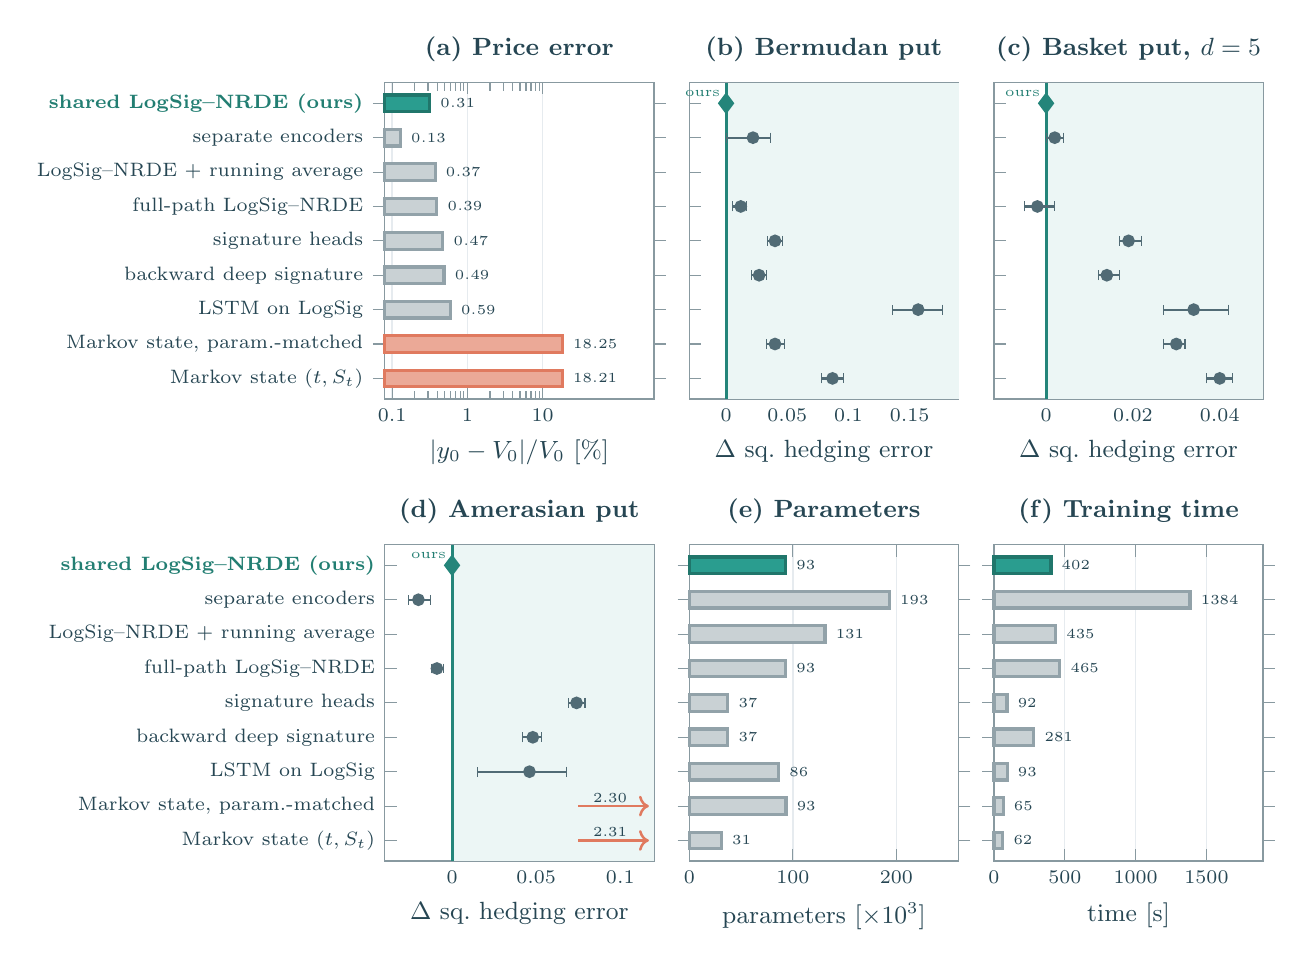
\begin{tikzpicture}
\pgfplotsset{forest/.style={paper, ymin=-0.6, ymax=8.6, y dir=reverse, ytick={0,...,8},
    ymajorgrids=false, xmajorgrids=true, axis lines*=box,
    xticklabel style={/pgf/number format/fixed}, scaled x ticks=false, clip=false},
  ci/.style={only marks, mark=*, mark size=1.7pt, color=cInk!80, mark options={fill=cInk!80},
    error bars/x dir=both, error bars/x explicit,
    error bars/error bar style={line width=0.8pt, color=cInk!80},
    error bars/error mark options={rotate=90, mark size=1.8pt, color=cInk!80}},
}
\begin{groupplot}[group style={group size=3 by 2, horizontal sep=0.45cm, vertical sep=1.85cm,
    yticklabels at=edge left},
  forest, width=5.0cm, height=5.6cm, yticklabels={{\textbf{\textcolor{cStop!80!black}{shared LogSig--NRDE (ours)}}},{separate encoders},{LogSig--NRDE + running average},{full-path LogSig--NRDE},{signature heads},{backward deep signature},{LSTM on LogSig},{Markov state, param.-matched},{Markov state $(t,S_t)$}},
  yticklabel style={font=\scriptsize, text=cInk}]
\nextgroupplot[title={(a) Price error}, xmode=log, xmin=0.08, xmax=300,
  xtick={0.1,1,10}, xticklabels={$0.1$,$1$,$10$}, xlabel={$|y_0-V_0|/V_0$ [\%]},
  xbar, bar width=6pt, bar shift=0pt, log origin=infty,
  nodes near coords, point meta=rawx, nodes near coords style={font=\tiny, text=cInk, anchor=west,
  xshift=0pt, /pgf/number format/.cd, fixed, precision=2}]
\addplot[fill=cStop, draw=cStop!75!black] coordinates {(0.3149,0)};
\addplot[fill=cInk!25, draw=cInk!50] coordinates {(0.1289,1) (0.3735,2) (0.3926,3) (0.4728,4) (0.4888,5) (0.5918,6)};
\addplot[fill=cJoint!65, draw=cJoint] coordinates {(18.252,7) (18.212,8)};
\nextgroupplot[title={(b) Bermudan put}, xmin=-0.03, xmax=0.19, xlabel={$\Delta$ sq.\ hedging error}]
\fill[cStop!9] (axis cs:0,\pgfkeysvalueof{/pgfplots/ymin}) rectangle (axis cs:\pgfkeysvalueof{/pgfplots/xmax},\pgfkeysvalueof{/pgfplots/ymax});
\draw[cStop!85!black, line width=1.1pt] (axis cs:0,\pgfkeysvalueof{/pgfplots/ymin}) -- (axis cs:0,\pgfkeysvalueof{/pgfplots/ymax});
\addplot[only marks, mark=diamond*, mark size=3pt, color=cStop!85!black] coordinates {(0,0)};
\addplot[ci] coordinates {(0.022,1) += (0.0140,0) -= (0.0220,0) (0.012,3) += (0.0050,0) -= (0.0070,0) (0.04,4) += (0.0060,0) -= (0.0060,0) (0.027,5) += (0.0060,0) -= (0.0060,0) (0.157,6) += (0.0200,0) -= (0.0210,0) (0.04,7) += (0.0080,0) -= (0.0070,0) (0.087,8) += (0.0090,0) -= (0.0090,0)};
\node[font=\tiny, text=cInk, anchor=north east, inner sep=2pt] at (axis cs:0,-0.55) {\textcolor{cStop!80!black}{ours}};
\nextgroupplot[title={(c) Basket put, $d=5$}, xmin=-0.012, xmax=0.05, xlabel={$\Delta$ sq.\ hedging error}]
\fill[cStop!9] (axis cs:0,\pgfkeysvalueof{/pgfplots/ymin}) rectangle (axis cs:\pgfkeysvalueof{/pgfplots/xmax},\pgfkeysvalueof{/pgfplots/ymax});
\draw[cStop!85!black, line width=1.1pt] (axis cs:0,\pgfkeysvalueof{/pgfplots/ymin}) -- (axis cs:0,\pgfkeysvalueof{/pgfplots/ymax});
\addplot[only marks, mark=diamond*, mark size=3pt, color=cStop!85!black] coordinates {(0,0)};
\addplot[ci] coordinates {(0.002,1) += (0.0020,0) -= (0.0020,0) (-0.002,3) += (0.0040,0) -= (0.0030,0) (0.019,4) += (0.0030,0) -= (0.0020,0) (0.014,5) += (0.0030,0) -= (0.0020,0) (0.034,6) += (0.0080,0) -= (0.0070,0) (0.03,7) += (0.0020,0) -= (0.0030,0) (0.04,8) += (0.0030,0) -= (0.0030,0)};
\node[font=\tiny, text=cInk, anchor=north east, inner sep=2pt] at (axis cs:0,-0.55) {\textcolor{cStop!80!black}{ours}};
\nextgroupplot[title={(d) Amerasian put}, xmin=-0.04, xmax=0.12, xlabel={$\Delta$ sq.\ hedging error}]
\fill[cStop!9] (axis cs:0,\pgfkeysvalueof{/pgfplots/ymin}) rectangle (axis cs:\pgfkeysvalueof{/pgfplots/xmax},\pgfkeysvalueof{/pgfplots/ymax});
\draw[cStop!85!black, line width=1.1pt] (axis cs:0,\pgfkeysvalueof{/pgfplots/ymin}) -- (axis cs:0,\pgfkeysvalueof{/pgfplots/ymax});
\addplot[only marks, mark=diamond*, mark size=3pt, color=cStop!85!black] coordinates {(0,0)};
\addplot[ci] coordinates {(-0.02,1) += (0.0070,0) -= (0.0060,0) (-0.009,3) += (0.0040,0) -= (0.0030,0) (0.074,4) += (0.0050,0) -= (0.0050,0) (0.048,5) += (0.0050,0) -= (0.0060,0) (0.046,6) += (0.0220,0) -= (0.0310,0)};
\draw[->, cJoint, line width=0.9pt] (axis cs:0.075,7) -- (axis cs:0.117,7) node[pos=0.45, above, font=\tiny, text=cInk, inner sep=1pt] {2.30};
\draw[->, cJoint, line width=0.9pt] (axis cs:0.075,8) -- (axis cs:0.117,8) node[pos=0.45, above, font=\tiny, text=cInk, inner sep=1pt] {2.31};
\node[font=\tiny, text=cInk, anchor=north east, inner sep=2pt] at (axis cs:0,-0.55) {\textcolor{cStop!80!black}{ours}};
\nextgroupplot[title={(e) Parameters}, xmin=0, xmax=260, xlabel={parameters [$\times10^{3}$]},
  xbar, bar width=6pt, bar shift=0pt, nodes near coords, point meta=rawx,
  nodes near coords style={font=\tiny, text=cInk, anchor=west, /pgf/number format/.cd, fixed, precision=0}]
\addplot[fill=cStop, draw=cStop!75!black] coordinates {(93.001,0)};
\addplot[fill=cInk!25, draw=cInk!50] coordinates {(193.225,1) (130.953,2) (93.001,3) (37.193,4) (37.194,5) (86.217,6) (93.347,7) (30.921,8)};
\nextgroupplot[title={(f) Training time}, xmin=0, xmax=1900, xticklabel style={/pgf/number format/1000 sep={}}, xlabel={time [s]},
  xbar, bar width=6pt, bar shift=0pt, nodes near coords, point meta=rawx,
  nodes near coords style={font=\tiny, text=cInk, anchor=west, /pgf/number format/.cd, fixed, precision=0, 1000 sep={}}]
\addplot[fill=cStop, draw=cStop!75!black] coordinates {(402,0)};
\addplot[fill=cInk!25, draw=cInk!50] coordinates {(1384,1) (435,2) (465,3) (92,4) (281,5) (93,6) (65,7) (62,8)};
\end{groupplot}
\end{tikzpicture}
}
\caption{Path encoders ($K=4$). (a) Relative price error on the Amerasian put, logarithmic scale. (b)--(d) Squared hedging error minus that of the shared LogSig--NRDE, with $95\pct$ interval; the shaded side favors our model. (e), (f) Model size and training time on the Amerasian put.}
\label{fig:encoders}
\end{figure}

Path information also improves hedging for Markovian problems (\cref{fig:encoders}b--d). All alternative encoders yield larger hedging errors on the Bermudan put, and on the five-asset basket put only the full-path LogSig--NRDE matches our shared local encoder. Moreover, sharing one encoder across layers is computationally decisive: compared with layer-specific encoders, it uses less than half the parameters and cuts training time by a factor of $3.4$ on the Amerasian put (\cref{fig:encoders}e,f), needs $162\,649$ instead of $463\,321$ parameters on the basket put, and delivers nearly identical primal--dual bounds.


%----------------------------------------------------------------------
\subsection{Rough volatility}\label{sec:exp-rough}
%----------------------------------------------------------------------

The rough Bergomi model \cite{bayer2016} with $H=0.07$, $\eta=1.9$, $\rho=-0.9$, and $\xi_0=0.09$ violates \cref{ass:obs}, since the price is no longer a Markov state and the spot variance is unobserved. \Cref{fig:rough} compares encoders and regression methods for the Bermudan put. Using only the price path, the LogSig--NRDE model attains tighter dual bounds than the Markov-state encoder and signature Longstaff--Schwartz, with equal or better lower bounds. Adding the spot variance as an input channel tightens the certificate further. Even then, the LogSig--NRDE encoder improves on the Markov state augmented with the variance, so the path encoder captures information beyond the current state when the variance is known.

\begin{figure}[htbp]
\centering
\resizebox{\textwidth}{!}{% Rough Bergomi Bermudan put: bounds of each method minus those of LogSig--NRDE, 95% intervals.
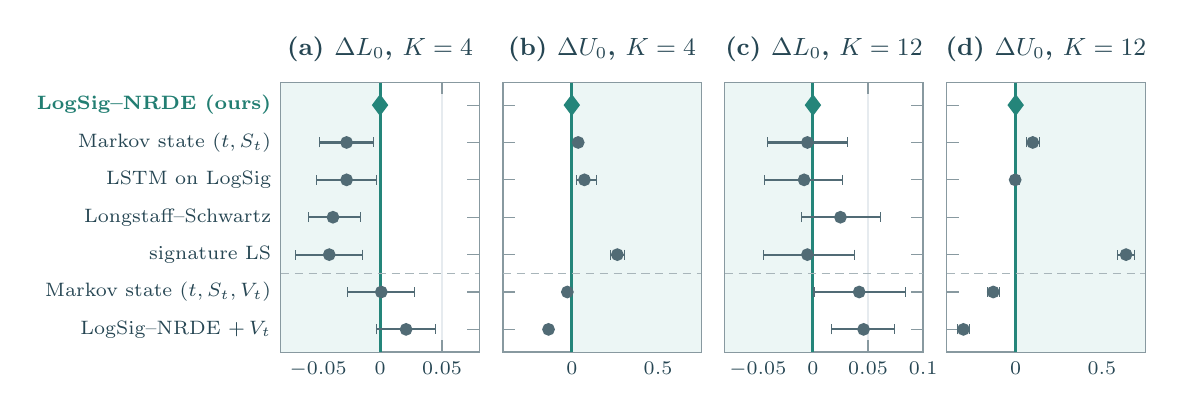
\begin{tikzpicture}
\pgfplotsset{forest/.style={paper, ymin=-0.6, ymax=6.6, y dir=reverse, ytick={0,...,6},
    ymajorgrids=false, xmajorgrids=true, axis lines*=box,
    xticklabel style={/pgf/number format/fixed}, scaled x ticks=false, clip=false},
  ci/.style={only marks, mark=*, mark size=1.7pt, color=cInk!80, mark options={fill=cInk!80},
    error bars/x dir=both, error bars/x explicit,
    error bars/error bar style={line width=0.8pt, color=cInk!80},
    error bars/error mark options={rotate=90, mark size=1.8pt, color=cInk!80}},
}
\begin{groupplot}[group style={group size=4 by 1, horizontal sep=0.3cm, yticklabels at=edge left},
  forest, width=4.1cm, height=5.0cm, yticklabels={{\textbf{\textcolor{cStop!80!black}{LogSig--NRDE (ours)}}},{Markov state $(t,S_t)$},{LSTM on LogSig},{Longstaff--Schwartz},{signature LS},{Markov state $(t,S_t,V_t)$},{LogSig--NRDE $+\,V_t$}}, yticklabel style={font=\scriptsize, text=cInk}]
\nextgroupplot[title={(a) $\Delta L_0$, $K=4$}, xmin=-0.08, xmax=0.08]
\fill[cStop!9] (axis cs:\pgfkeysvalueof{/pgfplots/xmin},\pgfkeysvalueof{/pgfplots/ymin}) rectangle (axis cs:0,\pgfkeysvalueof{/pgfplots/ymax});
\draw[cStop!85!black, line width=1.1pt] (axis cs:0,\pgfkeysvalueof{/pgfplots/ymin}) -- (axis cs:0,\pgfkeysvalueof{/pgfplots/ymax});
\addplot[only marks, mark=diamond*, mark size=3pt, color=cStop!85!black] coordinates {(0,0)};
\draw[cInk!40, densely dashed, line width=0.5pt] (axis cs:\pgfkeysvalueof{/pgfplots/xmin},4.5) -- (axis cs:\pgfkeysvalueof{/pgfplots/xmax},4.5);
\addplot[ci] coordinates {(-0.027,1) += (0.0220,0) -= (0.0220,0) (-0.027,2) += (0.0240,0) -= (0.0240,0) (-0.038,3) += (0.0220,0) -= (0.0200,0) (-0.041,4) += (0.0270,0) -= (0.0270,0) (0.001,5) += (0.0270,0) -= (0.0270,0) (0.021,6) += (0.0240,0) -= (0.0240,0)};
\nextgroupplot[title={(b) $\Delta U_0$, $K=4$}, xmin=-0.4, xmax=0.75]
\fill[cStop!9] (axis cs:0,\pgfkeysvalueof{/pgfplots/ymin}) rectangle (axis cs:\pgfkeysvalueof{/pgfplots/xmax},\pgfkeysvalueof{/pgfplots/ymax});
\draw[cStop!85!black, line width=1.1pt] (axis cs:0,\pgfkeysvalueof{/pgfplots/ymin}) -- (axis cs:0,\pgfkeysvalueof{/pgfplots/ymax});
\addplot[only marks, mark=diamond*, mark size=3pt, color=cStop!85!black] coordinates {(0,0)};
\draw[cInk!40, densely dashed, line width=0.5pt] (axis cs:\pgfkeysvalueof{/pgfplots/xmin},4.5) -- (axis cs:\pgfkeysvalueof{/pgfplots/xmax},4.5);
\addplot[ci] coordinates {(0.037,1) += (0.0140,0) -= (0.0150,0) (0.073,2) += (0.0710,0) -= (0.0480,0) (0.264,4) += (0.0420,0) -= (0.0400,0) (-0.026,5) += (0.0170,0) -= (0.0180,0) (-0.135,6) += (0.0160,0) -= (0.0160,0)};
\nextgroupplot[title={(c) $\Delta L_0$, $K=12$}, xmin=-0.08, xmax=0.1]
\fill[cStop!9] (axis cs:\pgfkeysvalueof{/pgfplots/xmin},\pgfkeysvalueof{/pgfplots/ymin}) rectangle (axis cs:0,\pgfkeysvalueof{/pgfplots/ymax});
\draw[cStop!85!black, line width=1.1pt] (axis cs:0,\pgfkeysvalueof{/pgfplots/ymin}) -- (axis cs:0,\pgfkeysvalueof{/pgfplots/ymax});
\addplot[only marks, mark=diamond*, mark size=3pt, color=cStop!85!black] coordinates {(0,0)};
\draw[cInk!40, densely dashed, line width=0.5pt] (axis cs:\pgfkeysvalueof{/pgfplots/xmin},4.5) -- (axis cs:\pgfkeysvalueof{/pgfplots/xmax},4.5);
\addplot[ci] coordinates {(-0.005,1) += (0.0360,0) -= (0.0360,0) (-0.008,2) += (0.0350,0) -= (0.0360,0) (0.025,3) += (0.0360,0) -= (0.0350,0) (-0.005,4) += (0.0430,0) -= (0.0400,0) (0.042,5) += (0.0420,0) -= (0.0410,0) (0.046,6) += (0.0280,0) -= (0.0290,0)};
\nextgroupplot[title={(d) $\Delta U_0$, $K=12$}, xmin=-0.4, xmax=0.75]
\fill[cStop!9] (axis cs:0,\pgfkeysvalueof{/pgfplots/ymin}) rectangle (axis cs:\pgfkeysvalueof{/pgfplots/xmax},\pgfkeysvalueof{/pgfplots/ymax});
\draw[cStop!85!black, line width=1.1pt] (axis cs:0,\pgfkeysvalueof{/pgfplots/ymin}) -- (axis cs:0,\pgfkeysvalueof{/pgfplots/ymax});
\addplot[only marks, mark=diamond*, mark size=3pt, color=cStop!85!black] coordinates {(0,0)};
\draw[cInk!40, densely dashed, line width=0.5pt] (axis cs:\pgfkeysvalueof{/pgfplots/xmin},4.5) -- (axis cs:\pgfkeysvalueof{/pgfplots/xmax},4.5);
\addplot[ci] coordinates {(0.099,1) += (0.0370,0) -= (0.0360,0) (-0.003,2) += (0.0250,0) -= (0.0220,0) (0.64,4) += (0.0500,0) -= (0.0500,0) (-0.13,5) += (0.0350,0) -= (0.0340,0) (-0.303,6) += (0.0340,0) -= (0.0350,0)};
\end{groupplot}
\end{tikzpicture}
}
\caption{Rough Bergomi Bermudan put ($\kappa=100$): bounds of each method minus those of the LogSig--NRDE model on the price path, with $95\pct$ interval; the shaded side favors the LogSig--NRDE model. Reference model: $[L_0,U_0]=[8.496,10.643]$ for $K=4$ and $[8.507,11.704]$ for $K=12$.}
\label{fig:rough}
\end{figure}

%----------------------------------------------------------------------
\subsection{Certificates and benchmarks}\label{sec:exp-benchmarks}
%----------------------------------------------------------------------

Every trained model yields a lower and an upper price bound (\cref{thm:primaldual}). Each reference value lies within two standard errors of the certified interval (\cref{tab:certificates}), and the interval narrows as the learning step decreases, as \cref{thm:primaldual}(b) predicts.

\begin{table}[htbp]
\centering\footnotesize
\caption{Prices and primal--dual certificates of the stop-gradient LogSig--NRDE model; standard errors in parentheses.}
\label{tab:certificates}
\setlength{\tabcolsep}{4pt}
\begin{tabular}{@{}l l c c c c c@{}}
\toprule
Contract & & Reference & $y_0$ & $L_0$ & $U_0$ & width [\%]\\
\midrule
\multirow{3}{*}{Bermudan put, $K=4$} & $\kappa=90$  & 2.4117 & 2.4146 & 2.4104 {\scriptsize(0.005)} & 2.4945 {\scriptsize(0.005)} & 3.5\\
                                     & $\kappa=100$ & 5.9566 & 5.9616 & 5.9508 {\scriptsize(0.010)} & 6.0683 {\scriptsize(0.006)} & 2.0\\
                                     & $\kappa=110$ & 11.7243 & 11.7321 & 11.7124 {\scriptsize(0.015)} & 11.8696 {\scriptsize(0.006)} & 1.3\\
Amerasian put, $K=4$ & & 3.7611 & 3.7729 & 3.7620 {\scriptsize(0.008)} & 3.7917 {\scriptsize(0.005)} & 0.8\\
Basket put, $d=5$, $K=4$ & & -- & 3.4885 & 3.4951 {\scriptsize(0.010)} & 3.5689 {\scriptsize(0.004)} & 2.1\\
\midrule
\multirow{3}{*}{Max-call, $d=2$, $K=9$} & $S_0=90$  & 8.075 & 8.090 & 8.099 {\scriptsize(0.027)} & 8.519 {\scriptsize(0.014)} & 5.2\\
                                        & $S_0=100$ & 13.902 & 13.921 & 13.934 {\scriptsize(0.034)} & 14.524 {\scriptsize(0.017)} & 4.2\\
                                        & $S_0=110$ & 21.345 & 21.364 & 21.372 {\scriptsize(0.039)} & 22.178 {\scriptsize(0.019)} & 3.8\\
\multirow{3}{*}{Max-call, $d=5$, $K=9$} & $S_0=90$  & 16.644 & 16.697 & 16.633 {\scriptsize(0.036)} & 17.357 {\scriptsize(0.020)} & 4.3\\
                                        & $S_0=100$ & 26.159 & 26.237 & 26.143 {\scriptsize(0.044)} & 27.116 {\scriptsize(0.023)} & 3.7\\
                                        & $S_0=110$ & 36.772 & 36.875 & 36.755 {\scriptsize(0.049)} & 37.956 {\scriptsize(0.026)} & 3.3\\
\bottomrule
\end{tabular}
\end{table}

The LogSig--NRDE policy is never dominated by Longstaff--Schwartz regression \cite{longstaff2001}, deep optimal stopping \cite{becker2019}, or signature Longstaff--Schwartz \cite{bayer2025primal} (\cref{fig:benchmarks}). Its advantage over regression grows with the dimension, and its dual bound is markedly tighter than the signature-based dual bound.

\begin{figure}[htbp]
\centering
\resizebox{\textwidth}{!}{% Benchmarks on common paths: bound of each benchmark minus that of LogSig--NRDE, 95% intervals.
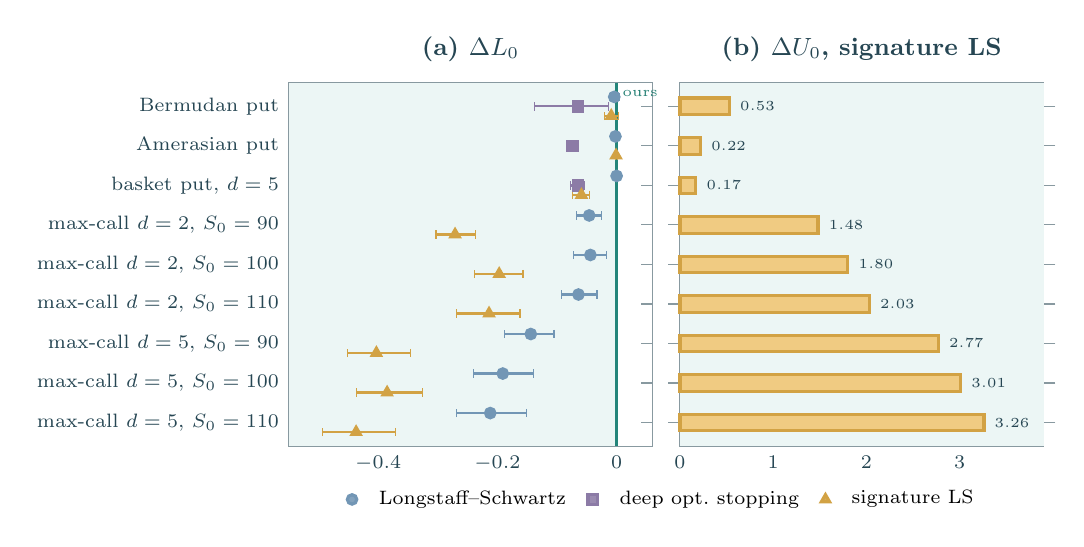
\begin{tikzpicture}
\pgfplotsset{forest/.style={paper, ymin=-0.6, ymax=8.6, y dir=reverse, ytick={0,...,8},
    ymajorgrids=false, xmajorgrids=true, axis lines*=box,
    xticklabel style={/pgf/number format/fixed}, scaled x ticks=false, clip=false},
  ci/.style={only marks, mark=*, mark size=1.7pt, color=cInk!80, mark options={fill=cInk!80},
    error bars/x dir=both, error bars/x explicit,
    error bars/error bar style={line width=0.8pt, color=cInk!80},
    error bars/error mark options={rotate=90, mark size=1.8pt, color=cInk!80}},
}
\begin{groupplot}[group style={group size=2 by 1, horizontal sep=0.35cm, yticklabels at=edge left},
  forest, ymin=-0.6, width=6.2cm, height=6.2cm, yticklabels={{Bermudan put},{Amerasian put},{basket put, $d=5$},{max-call $d=2$, $S_0=90$},{max-call $d=2$, $S_0=100$},{max-call $d=2$, $S_0=110$},{max-call $d=5$, $S_0=90$},{max-call $d=5$, $S_0=100$},{max-call $d=5$, $S_0=110$}}, yticklabel style={font=\scriptsize, text=cInk}]
\nextgroupplot[title={(a) $\Delta L_0$}, xmin=-0.55, xmax=0.06,
  legend style={at={(1.03,-0.09)}, anchor=north, font=\scriptsize, legend columns=3, column sep=6pt}]
\fill[cStop!9] (axis cs:\pgfkeysvalueof{/pgfplots/xmin},\pgfkeysvalueof{/pgfplots/ymin}) rectangle (axis cs:0,\pgfkeysvalueof{/pgfplots/ymax});
\draw[cStop!85!black, line width=1.1pt] (axis cs:0,\pgfkeysvalueof{/pgfplots/ymin}) -- (axis cs:0,\pgfkeysvalueof{/pgfplots/ymax});
\addplot[ci, color=cFull!90!black, mark=*, mark options={fill=cFull!90!black}, error bars/error bar style={color=cFull!90!black}, error bars/error mark options={rotate=90, mark size=1.5pt, color=cFull!90!black}] coordinates {(-0.004,-0.24) += (0.0080,0) -= (0.0080,0) (-0.002,0.76) += (0.0020,0) -= (0.0020,0) (0.0,1.76) += (0.0060,0) -= (0.0060,0) (-0.046,2.76) += (0.0200,0) -= (0.0210,0) (-0.044,3.76) += (0.0270,0) -= (0.0280,0) (-0.064,4.76) += (0.0310,0) -= (0.0280,0) (-0.144,5.76) += (0.0390,0) -= (0.0440,0) (-0.191,6.76) += (0.0520,0) -= (0.0490,0) (-0.212,7.76) += (0.0610,0) -= (0.0570,0)};
\addlegendentry{Longstaff--Schwartz}
\addplot[ci, color=cEma!90!black, mark=square*, mark options={fill=cEma!90!black}, error bars/error bar style={color=cEma!90!black}, error bars/error mark options={rotate=90, mark size=1.5pt, color=cEma!90!black}] coordinates {(-0.065,0.0) += (0.0510,0) -= (0.0730,0) (-0.074,1.0) += (0.0060,0) -= (0.0060,0) (-0.065,2.0) += (0.0110,0) -= (0.0120,0)};
\addlegendentry{deep opt.\ stopping}
\addplot[ci, color=cLayer!90!black, mark=triangle*, mark options={fill=cLayer!90!black}, error bars/error bar style={color=cLayer!90!black}, error bars/error mark options={rotate=90, mark size=1.5pt, color=cLayer!90!black}] coordinates {(-0.009,0.24) += (0.0120,0) -= (0.0110,0) (-0.001,1.24) += (0.0020,0) -= (0.0010,0) (-0.059,2.24) += (0.0140,0) -= (0.0150,0) (-0.271,3.24) += (0.0350,0) -= (0.0320,0) (-0.197,4.24) += (0.0400,0) -= (0.0420,0) (-0.214,5.24) += (0.0520,0) -= (0.0540,0) (-0.403,6.24) += (0.0570,0) -= (0.0490,0) (-0.385,7.24) += (0.0590,0) -= (0.0510,0) (-0.437,8.24) += (0.0660,0) -= (0.0570,0)};
\addlegendentry{signature LS}
\node[font=\tiny, anchor=north west, inner sep=2pt] at (axis cs:0,-0.55) {\textcolor{cStop!80!black}{ours}};
\nextgroupplot[title={(b) $\Delta U_0$, signature LS}, xmin=0, xmax=3.9,
  xbar, bar width=6pt, bar shift=0pt, nodes near coords, point meta=rawx,
  nodes near coords style={font=\tiny, text=cInk, anchor=west, /pgf/number format/.cd, fixed, zerofill, precision=2}]
\fill[cStop!9] (rel axis cs:0,0) rectangle (rel axis cs:1,1);
\addplot[fill=cLayer!70, draw=cLayer!90!black] coordinates {(0.53,0) (0.22,1) (0.17,2) (1.48,3) (1.8,4) (2.03,5) (2.77,6) (3.01,7) (3.26,8)};
\end{groupplot}
\end{tikzpicture}
}
\caption{Benchmarks on common paths: lower bound of each benchmark and upper bound of signature LS minus those of the LogSig--NRDE model, with $95\pct$ interval; the shaded side favors the LogSig--NRDE model. Deep optimal stopping was not run on the max-call.}
\label{fig:benchmarks}
\end{figure}

From one to ten assets, the certified interval of the basket put barely widens, and the geometric basket call retains its accuracy (\cref{fig:dim}). The model size grows with the dimension of the local log-signature, while the training time stays between $290$ and $920$\,s across all dimensions (\cref{fig:dim}c).

\begin{figure}[htbp]
\centering
\resizebox{\textwidth}{!}{% Dimension d = 1, 2, 5, 10 (M = 2): certified interval width of the
% Bermudan basket put, price error of the geometric basket call, size.
\begin{tikzpicture}
\begin{groupplot}[group style={group size=3 by 1, horizontal sep=1.5cm},
                  paper, width=5.6cm, height=5.0cm,
                  xmode=log, xmin=0.8, xmax=12.5, xtick={1,2,5,10},
                  xticklabels={$1$,$2$,$5$,$10$}, xlabel={dimension $d$}]
\nextgroupplot[title={(a) Accuracy}, ylabel={[\%]}, ymin=0, ymax=3,
               legend style={at={(0.97,0.36)}, anchor=east}]
\addplot[sStop] table[x=d, y=berm_relgap] {data/dim.dat};
\addplot[color=cEma, mark=diamond*, mark size=2.6pt] table[x=d, y=geo_err] {data/dim.dat};
\legend{put: $(U_0-L_0)/L_0$, call: $|y_0-V_0|/V_0$}

\nextgroupplot[title={(b) Model size}, ylabel={parameters [$\times10^{5}$]},
               ymin=0, ymax=5.2, ytick={0,1,...,5}, legend style={at={(0.03,0.97)}, anchor=north west}]
\addplot[sStop] table[x=d, y expr=\thisrow{berm_params}/1e5] {data/dim.dat};
\addplot[color=cEma, mark=diamond*, mark size=2.6pt] table[x=d, y expr=\thisrow{geo_params}/1e5] {data/dim.dat};
\legend{Bermudan put ($K=4$), geometric call ($K=1$)}

\nextgroupplot[title={(c) Training time}, ylabel={time [s]},
               ymin=0, ymax=1000, legend style={at={(0.03,0.97)}, anchor=north west}]
\addplot[sStop] table[x=d, y=berm_time] {data/dim.dat};
\addplot[color=cEma, mark=diamond*, mark size=2.6pt] table[x=d, y=geo_time] {data/dim.dat};
\legend{Bermudan put, geometric call}
\end{groupplot}
\end{tikzpicture}
}
\caption{Dimension scaling at $M=2$. (a) Relative width of the certified interval (Bermudan basket put, $K=4$) and relative price error (geometric basket call). (b) Number of parameters. (c) Training time.}
\label{fig:dim}
\end{figure}

%======================================================================
\FloatBarrier
\section{Conclusion}\label{sec:conclusion}
%======================================================================

We extended the compound BSDE to path-dependent contracts with early exercise and showed how its interfaces should be trained. A single log-signature Neural RDE encodes the price path for all layers. Detaching the interface target turns every value head into the conditional expectation of its target, so the stationary price coincides with the optimal stopping value under the encoder filtration, whereas joint differentiation of the target shifts this price by a residual-driven bias that persists at every training budget. Moreover, the training loss controls the price and hedge errors without a smallness condition, the total error splits into four separately controlled terms, and the trained network certifies its own price through primal--dual bounds. The experiments confirm each of these statements and show that stop-gradient training reduces the price error of joint training by one to two orders of magnitude at equal cost.

Several directions remain open for future research. First, while our experiments indicate that the joint-training bias decays at first order in the learning step $h$, a rigorous convergence rate remains to be established. Second, in the continuous-exercise limit $K\to\infty$, the compound BSDE should converge to a reflected BSDE, which requires refining our error bounds to remove the explicit factor of $K$. Third, for non-Markovian dynamics such as the rough Bergomi model, \cref{ass:obs} no longer holds; although the log-signature encoder still tightens the primal--dual certificates in practice (\cref{sec:exp-rough}), extending the information analysis of \cref{lem:information} to rough volatility requires characterizing an appropriate infinite-dimensional state.


\appendix
%======================================================================
\FloatBarrier
\section{Proofs}\label{app:proofs}
%======================================================================

\subsection{Discounting}\label{app:discount}

\begin{lemma}[discounting]\label{lem:discount}
\leavevmode
\begin{enumerate}[label=(\roman*)]
\item $(Y,Z)$ solves \eqref{eq:cbsde} if and only if $(e^{-rt}Y_t,e^{-rt}Z_t)$ solves \eqref{eq:cbsde} with $r=0$ and links $\tilde g_j(x,y)=e^{-rT_j}g_j(x,e^{rT_j}y)$. If $g_j$ satisfies \cref{ass:link}, so does $\tilde g_j$, with constant $e^{-rT_j}L_g\le L_g$.
\item Let $\beta_i=(1+rh)^{-i}$. The undiscounted step $\hY_{j,u_{i+1}}=(1+rh)\hY_{j,u_i}+\hZ_{u_i}^\top\Delta W_i$ is equivalent to
\[
\beta_{i+1}\hY_{j,u_{i+1}}=\beta_i\hY_{j,u_i}+\left(\beta_{i+1}\hZ_{u_i}\right)^\top\Delta W_i ,
\]
an exact martingale transform for every choice of $\hZ$. Moreover $1\le\beta_ie^{ru_i}\le e^{r^2u_ih/2}$.
\end{enumerate}
\end{lemma}

\begin{proof}
(i) On layer $j$, we have $\dd Y_{j,t}=rY_{j,t}\dd t+Z_{j,t}^\top\dd W_t$. Applying It\^o's formula, we obtain $\dd(e^{-rt}Y_{j,t})=e^{-rt}Z_{j,t}^\top\dd W_t$. At the interface, the link condition reads
\[
e^{-rT_j}Y_{j,T_j}=e^{-rT_j}g_j\left(S_{[0,T_j]},e^{rT_j}e^{-rT_j}Y_{j+1,T_j}\right)=\tilde g_j\left(S_{[0,T_j]},e^{-rT_j}Y_{j+1,T_j}\right).
\]
Multiplying by $e^{rt}$ reverses the argument and proves the converse. For the Lipschitz constant, \cref{ass:link} implies
\begin{align*}
\abs{\tilde g_j(x,y)-\tilde g_j(x',y')}&\le e^{-rT_j}\max\bigl\{L_g\norm{x-x'}_{T_j},e^{rT_j}\abs{y-y'}\bigr\}\\
&=\max\bigl\{e^{-rT_j}L_g\norm{x-x'}_{T_j},\abs{y-y'}\bigr\}.
\end{align*}

(ii) Multiplying the undiscounted step by $\beta_{i+1}$, we arrive at the displayed recursion. Since $\E[\Delta W_i\mid\cF_{u_i}]=0$, the discounted values form a martingale. As $u_i=ih$, we can write $\beta_ie^{ru_i}=\exp(i[rh-\log(1+rh)])$. The elementary bound $0\le x-\log(1+x)\le x^2/2$ for $x\ge0$ then shows $0\le i[rh-\log(1+rh)]\le r^2u_ih/2$.
\end{proof}

The relative mismatch between $\beta_i$ and $e^{-ru_i}$ is at most $e^{r^2Th/2}-1=O(h)$ and adds $O(h^2)$ to every squared error below. It is not tracked further.

\subsection{Proof of \texorpdfstring{\cref{thm:wellposed}}{Theorem 1}}\label{app:wellposed}

\begin{proof}

Let $L$ denote the Lipschitz constant of $b$ and $\sigma$.

(i) \emph{Existence.} Under \cref{ass:sde}, \eqref{eq:sde} admits a unique strong solution with $\E\norm{S}_T^2<\infty$. Since $\abs{\Phi_K(S_{[0,T]})}\le\abs{\Phi_K(0)}+L_g\norm{S}_T$, the terminal payoff is square integrable. Define $Y_{K,t}=\E[\Phi_K(S_{[0,T]})\mid\cF_t]$ on $[T_{K-1},T]$. By the martingale representation theorem, there exists $Z_K$ with $Y_{K,t}=\Phi_K-\int_t^TZ_{K,s}^\top\dd W_s$. Suppose layer $j+1$ has been constructed. According to \cref{ass:link},
\[
\abs{g_j(S_{[0,T_j]},Y_{j+1,T_j})}\le\abs{g_j(0,0)}+L_g\norm{S}_{T_j}+\abs{Y_{j+1,T_j}},
\]
which shows that the terminal value of layer $j$ is square integrable. We define $Y_{j,t}=\E[g_j(S_{[0,T_j]},Y_{j+1,T_j})\mid\cF_t]$ and obtain $Z_j$ from the martingale representation theorem. By Doob's inequality and It\^o's isometry, we get
\[
\E\sup_{t\in[T_{j-1},T_j]}\abs{Y_{j,t}}^2\le4\E\abs{Y_{j,T_j}}^2,\quad
\E\int_{T_{j-1}}^{T_j}\abs{Z_{j,t}}^2\dd t=\E\abs{Y_{j,T_j}-Y_{j,T_{j-1}}}^2\le\E\abs{Y_{j,T_j}}^2 .
\]
\emph{Uniqueness.} Taking conditional expectations in the last layer, we find $Y_{K,t}=\E[\Phi_K\mid\cF_t]$ for every square-integrable solution. Two candidates $Z_K,Z_K'$ satisfy $\int_{T_{K-1}}^T(Z_{K,t}-Z'_{K,t})^\top\dd W_t=0$, and It\^o's isometry implies $Z_K=Z'_K$. Once layer $j+1$ is unique, the terminal value of layer $j$ is determined, and the same argument applies.

(ii) Define $u_K(t,x)=\E[\Phi_K(S^{t,x}_{[0,T]})]$ and $u_j$ recursively as in the statement. Given $\cF_t$, the past path is fixed, and the future depends only on $S_t$ and on the increments of $W$ after $t$, which are independent of $\cF_t$. We therefore obtain $\E[\Phi_K(S_{[0,T]})\mid\cF_t]=u_K(t,S_{[0,t]})$. If $Y_{j+1,T_j}=u_{j+1}(T_j,S_{[0,T_j]})$, the same argument shows $Y_{j,t}=u_j(t,S_{[0,t]})$.

(iii) Let $S=S^{t,x}$ and $S'=S^{t,x'}$. For $s\ge t$,
\[
S_s-S'_s=x_t-x'_t+\int_t^s[b(q,S_q)-b(q,S'_q)]\dd q+\int_t^s[\sigma(q,S_q)-\sigma(q,S'_q)]\dd W_q .
\]
Fix $v\in[t,T]$. By the Cauchy--Schwarz inequality, the squared supremum of the drift term is at most $TL^2\int_t^v\norm{S-S'}_q^2\dd q$. Doob's inequality and It\^o's isometry bound the expected squared supremum of the stochastic term by $4L^2\int_t^v\E\norm{S-S'}_q^2\dd q$. Using $\abs{a+b+c}^2\le3(\abs a^2+\abs b^2+\abs c^2)$, we deduce
\[
\E\norm{S-S'}_v^2\le3\norm{x-x'}_t^2+3L^2(T+4)\int_t^v\E\norm{S-S'}_q^2\dd q ,
\]
and Gronwall's inequality leads to $\E\norm{S-S'}_T\le\sqrt3\exp\left(\tfrac32L^2(T+4)T\right)\norm{x-x'}_t=:C\norm{x-x'}_t$. Let $F_j(y)=g_j(y,u_{j+1}(T_j,y))$ for $j<K$ and $F_K=\Phi_K$. Both paths are driven by the same Brownian motion, so the flow property yields $u_{j+1}(T_j,S_{[0,T_j]})=\E[F_{j+1}(S)\mid\cF_{T_j}]$, and likewise for $S'$. We claim that $\abs{F_j(S)-F_j(S')}\le L_g\E[\norm{S-S'}_T\mid\cF_{T_j}]$. The claim is immediate for $j=K$. Assuming it for $j+1$, we derive from \cref{ass:link}
\[
\begin{aligned}\abs{F_j(S)-F_j(S')}&\le\max\bigl\{L_g\norm{S-S'}_{T_j},\ \E[\abs{F_{j+1}(S)-F_{j+1}(S')}\mid\cF_{T_j}]\bigr\}\\&\le L_g\E[\norm{S-S'}_T\mid\cF_{T_j}] .\end{aligned}
\]
Taking expectations, we conclude $\abs{u_j(t,x)-u_j(t,x')}\le L_g\E\norm{S-S'}_T\le CL_g\norm{x-x'}_t$ for every $j$, where $C$ does not depend on $K$.

(iv) For Bermudan links, we have $Y_{k,T_k}=\max\{\Phi_k,\E[Y_{k+1,T_{k+1}}\mid\cF_{T_k}]\}$ and $Y_{K,T_K}=\Phi_K$. This is the Snell recursion, so $(Y_{k,T_k})$ is the smallest supermartingale dominating $(\Phi_k)$. Concatenating the layer martingales, we obtain
\[
Y_{k,T_k}-\int_0^{T_k}Z_s^\top\dd W_s=Y_{1,0}-\sum_{j=1}^{k-1}(Y_{j,T_j}-Y_{j+1,T_j})=Y_{1,0}-\sum_{j=1}^{k-1}\left(\Phi_j-Y_{j+1,T_j}\right)^+ .
\]
Since $\Phi_k\le Y_{k,T_k}$, this implies $\Phi_k-\int_0^{T_k}Z_s^\top\dd W_s\le Y_{1,0}$ for all $k$. On $\{\tau^*=T_k\}$, every earlier date satisfies $\Phi_j<Y_{j+1,T_j}$ and $\Phi_k=Y_{k,T_k}$, so equality holds at $k$. This establishes \eqref{eq:dual-identity}, and taking expectations at $\tau^*$ gives $V_0=\E\Phi_{\tau^*}=Y_{1,0}$.
\end{proof}

\subsection{Proof of \texorpdfstring{\cref{lem:nonanticipation}}{Lemma 3}}\label{app:nonanticipation}

\begin{proof}

(i) Each simulation step $S^{\mathrm f}_{t_{n+1}}$ is a Borel function of $S^{\mathrm f}_{t_n}$ and $W_{t_{n+1}}-W_{t_n}$. By induction over $n$, we get $\cG^{\pi}_{u_i}\subseteq\cF_{u_i}$. Each $\ell_k$ is a Borel function of the fine-grid prices on $[u_k,u_{k+1}]$, and $u_{k+1}\le u_i$ for $k<i$, which shows $\cG^{M}_{u_i}\subseteq\cG^{\pi}_{u_i}$. The complete Runge--Kutta update over one learning interval is a Borel map $H_{u_{i+1}}=R_\theta(H_{u_i},\ell_i)$. If $H_{u_i}$ is $\cG^{M}_{u_i}$-measurable, it follows that $H_{u_{i+1}}$ is $\cG^{M}_{u_{i+1}}$-measurable, and induction completes (i).

(ii) The heads take $\xi_i=(H_{u_i},X_{u_i})$ as input. The price part of $X_{u_i}$ equals $X_0$ plus the sum of the level-one price coordinates of $\ell_0,\dots,\ell_{i-1}$, and the time part is deterministic. Combined with (i), this shows that $\xi_i$, $\hZ_{u_i}$, and $\hY_{j,T_{j-1}}$ have the stated measurability.

(iii) Since $\Delta W_i$ is independent of $\cF_{u_i}$, we have $\E[\Delta W_i\mid\cF_{u_i}]=0$ and $\E[\Delta W_i\Delta W_i^\top\mid\cF_{u_i}]=hI_d$. Together with (ii), we obtain
\[
\E[\hY_{j,u_{i+1}}\mid\cF_{u_i}]=\hY_{j,u_i},\quad
\E[\abs{\hY_{j,u_{i+1}}}^2\mid\cF_{u_i}]=\abs{\hY_{j,u_i}}^2+h\abs{\hZ_{u_i}}^2 .
\]
Iterating this identity, we find $\E\abs{\hY_{j,u_i}}^2=\E\abs{\hY_{j,T_{j-1}}}^2+h\sum_{T_{j-1}\le u_k<u_i}\E\abs{\hZ_{u_k}}^2<\infty$. For the piecewise-constant integrand $\hZ_t=\sum_i\hZ_{u_i}\1_{(u_i,u_{i+1}]}(t)$, we have $\E\int_{T_{j-1}}^{T_j}\abs{\hZ_t}^2\dd t=h\sum_i\E\abs{\hZ_{u_i}}^2<\infty$. The stochastic integral is therefore a square-integrable martingale, and so is $\hY_{j,t}=\hY_{j,T_{j-1}}+\int_{T_{j-1}}^t\hZ_v^\top\dd W_v$.
\end{proof}

\subsection{Proof of \texorpdfstring{\cref{thm:discretisation}}{Theorem 4}}\label{app:discretisation}

\begin{proof}

We first show that $\bZ$ is optimal. Let $A\in L^2(\cF_{u_i};\R^d)$ and expand $\E\int_{u_i}^{u_{i+1}}\abs{Z_t-A}^2\dd t$ around $\bZ_{u_i}$. Conditioning on $\cF_{u_i}$, we find that the cross term equals
\[
\E\left[\left(\E\left[\int_{u_i}^{u_{i+1}}Z_t\dd t\Bigm|\cF_{u_i}\right]-h\bZ_{u_i}\right)^\top(A-\bZ_{u_i})\right]=0 .
\]
We thus obtain
\begin{equation}\label{eq:proj-best}
\E\int_{u_i}^{u_{i+1}}\abs{Z_t-A}^2\dd t=\E\int_{u_i}^{u_{i+1}}\abs{Z_t-\bZ_{u_i}}^2\dd t+h\,\E\abs{A-\bZ_{u_i}}^2 ,
\end{equation}
which shows $\varepsilon^\pi(Z)=\inf_{\hZ}\E\int_0^T\abs{Z_t-\hZ_t}^2\dd t$ over integrands that are constant and $\cF_{u_i}$-measurable on each $[u_i,u_{i+1})$.

(a) Let $D=L_g\norm{S-\Ipl S^{\mathrm f}}_T$. We claim $\abs{Y_{j,t}-Y^{\mathrm f}_{j,t}}\le\E[D\mid\cF_t]$ on every layer. At maturity, $\abs{Y_{K,T}-Y^{\mathrm f}_{K,T}}=\abs{\Phi_K(S)-\Phi_K(\Ipl S^{\mathrm f})}\le D$, and conditioning on $\cF_t$ proves the claim on layer $K$. Suppose the claim holds at $T_j$ for layer $j+1$. By \cref{ass:link}, we get
\[
\abs{Y_{j,T_j}-Y^{\mathrm f}_{j,T_j}}\le\max\bigl\{L_g\norm{S-\Ipl S^{\mathrm f}}_{T_j},\abs{Y_{j+1,T_j}-Y^{\mathrm f}_{j+1,T_j}}\bigr\}\le\E[D\mid\cF_{T_j}],
\]
because $L_g\norm{S-\Ipl S^{\mathrm f}}_{T_j}$ is $\cF_{T_j}$-measurable and bounded by $D$. Conditioning extends the claim to $[T_{j-1},T_j]$. By the conditional Jensen inequality, we obtain $\E\abs{Y_{j,t}-Y^{\mathrm f}_{j,t}}^2\le\E D^2=L_g^2\emon$. For the hedge, It\^o's isometry implies
\[
\E\int_{T_{j-1}}^{T_j}\abs{Z_{j,t}-Z^{\mathrm f}_{j,t}}^2\dd t=\E\abs{Y_{j,T_j}-Y^{\mathrm f}_{j,T_j}}^2-\E\abs{Y_{j,T_{j-1}}-Y^{\mathrm f}_{j,T_{j-1}}}^2\le L_g^2\emon ,
\]
and summing over $j$ completes the proof of (a).

(b) \emph{Monitoring.} Let $\underline S^{\mathrm f}_t=S^{\mathrm f}_{t_n}$ on $[t_n,t_{n+1})$. Under \cref{ass:sde}, \cite[Thm.~4.2]{zhang2004} shows $\E\norm{S-\underline S^{\mathrm f}}_T^2\le C\hf\log(2T/\hf)$. It remains to pass to the interpolation. On each fine interval we have $\norm{\Ipl S^{\mathrm f}-\underline S^{\mathrm f}}\le\max_n\abs{S^{\mathrm f}_{t_{n+1}}-S^{\mathrm f}_{t_n}}$, and
\[
\abs{S^{\mathrm f}_{t_{n+1}}-S^{\mathrm f}_{t_n}}\le\abs{S^{\mathrm f}_{t_{n+1}}-S_{t_{n+1}}}+\lim_{t\uparrow t_{n+1}}\abs{S_t-\underline S^{\mathrm f}_t}\le2\norm{S-\underline S^{\mathrm f}}_T .
\]
By the triangle inequality, we deduce $\norm{S-\Ipl S^{\mathrm f}}_T\le3\norm{S-\underline S^{\mathrm f}}_T$, and hence $\emon\le9\E\norm{S-\underline S^{\mathrm f}}_T^2\le C\hf\log(2T/\hf)$.

\emph{Grid regularity.} Let $F_j(x)=g_j(x,u_{j+1}(T_j,x))$ for $j<K$ and $F_K=\Phi_K$. From \cref{ass:link} and \cref{thm:wellposed}(iii), we get $\abs{F_j(x)-F_j(x')}\le CL_g\norm{x-x'}_{T_j}$. Subtracting a constant does not change the integrand, so we may assume $F_j(0)=0$. Let $\tilde Z_j$ be the integrand of $\E[F_j(S)\mid\cF_t]=\E F_j(S)+\int_0^t\tilde Z_{j,s}^\top\dd W_s$ on $[0,T]$. Uniqueness in the martingale representation shows $\tilde Z_j=Z_j$ on $[T_{j-1},T_j]$. Take smooth coefficients $b^{(n)},\sigma^{(n)}$ and smooth functionals $F^{(n)}_j$ of finitely many path values with $\E\norm{S^{(n)}-S}_T^2\to0$, $F_j^{(n)}(0)=0$, $\abs{F_j^{(n)}(x)-F_j^{(n)}(x')}\le CL_g\norm{x-x'}_T$, and $F_j^{(n)}\to F_j$ pointwise \cite{zhang2004}. By the Lipschitz property, we have
\[
\norm{F_j^{(n)}(S^{(n)})-F_j(S)}_{L^2}\le CL_g\left(\E\norm{S^{(n)}-S}_T^2\right)^{1/2}+\norm{F_j^{(n)}(S)-F_j(S)}_{L^2}\to0,
\]
where the second term vanishes by dominated convergence with the bound $2CL_g\norm{S}_T$. It\^o's isometry then implies $\E\int_0^T\abs{\tilde Z^{(n)}_{j,t}-\tilde Z_{j,t}}^2\dd t\to0$. For the smooth problems, Zhang's regularity theorem \cite{zhang2004} provides $\sum_i\E\int_{u_i}^{u_{i+1}}\abs{\tilde Z^{(n)}_{j,t}-\tilde Z^{(n)}_{j,u_i}}^2\dd t\le Ch$, and \eqref{eq:proj-best} reduces this to $\varepsilon^\pi(\tilde Z^{(n)}_j)\le Ch$. Since $Z\mapsto Z-\bZ$ is an orthogonal projection in $L^2$, we find
\[
\Bigl\lvert\sqrt{\varepsilon^\pi(\tilde Z^{(n)}_j)}-\sqrt{\varepsilon^\pi(\tilde Z_j)}\Bigr\rvert\le\left(\E\int_0^T\abs{\tilde Z^{(n)}_{j,t}-\tilde Z_{j,t}}^2\dd t\right)^{1/2}\to0 .
\]
Letting $n\to\infty$, we obtain $\varepsilon^\pi(Z_j)\le Ch$ on each layer. Summing over $j$, we conclude $\varepsilon^\pi(Z)\le CKh$.
\end{proof}

\subsection{Proof of \texorpdfstring{\cref{thm:aposteriori}}{Theorem 5}}\label{app:aposteriori}

\begin{proof}

Let $\delta Y_{j,t}=Y^{\mathrm f}_{j,t}-\hY_{j,t}$ and $\delta Z_{j,t}=Z^{\mathrm f}_{j,t}-\hZ_t$. Both processes are martingales on layer $j$, so $\delta Y_{j,t}=\delta Y_{j,T_{j-1}}+\int_{T_{j-1}}^t\delta Z_{j,s}^\top\dd W_s$. By It\^o's isometry, we obtain
\[
\E\abs{\delta Y_{j,t}}^2=\E\abs{\delta Y_{j,T_{j-1}}}^2+\E\int_{T_{j-1}}^t\abs{\delta Z_{j,s}}^2\dd s .
\]
This identity shows $\sup_t\E\abs{\delta Y_{j,t}}^2=\E\abs{\delta Y_{j,T_j}}^2$ and $\E\int_{T_{j-1}}^{T_j}\abs{\delta Z_{j,t}}^2\dd t=\norm{\delta Y_{j,T_j}}_{L^2}^2-\norm{\delta Y_{j,T_{j-1}}}_{L^2}^2$. At maturity, $\delta Y_{K,T}=-e_K$. For $j<K$, the definition of the residual gives
\[
\delta Y_{j,T_j}=g^{\mathrm f}_j(Y^{\mathrm f}_{j+1,T_j})-g^{\mathrm f}_j(\hY_{j+1,T_j})-e_j,
\]
and the $1$-Lipschitz property of the link in $y$ implies
\[
\norm{\delta Y_{j,T_j}}_{L^2}\le\norm{\delta Y_{j+1,T_j}}_{L^2}+\norm{e_j}_{L^2}\le\norm{\delta Y_{j+1,T_{j+1}}}_{L^2}+\norm{e_j}_{L^2}.
\]
By backward induction, we get $\norm{\delta Y_{j,T_j}}_{L^2}\le\sum_{k\ge j}\norm{e_k}_{L^2}$. The Cauchy--Schwarz inequality then shows $\max_j\sup_t\E\abs{\delta Y_{j,t}}^2\le(\sum_k\norm{e_k}_{L^2})^2\le K\cL(\theta)$. Telescoping the isometries over the layers, we derive
\begin{align*}
\abs{y_0-V^{\mathrm f}_0}^2+\sum_{j=1}^K\E\int_{T_{j-1}}^{T_j}\abs{\delta Z_{j,t}}^2\dd t
&=\norm{e_K}_{L^2}^2+\sum_{j=1}^{K-1}\left(\norm{\delta Y_{j,T_j}}_{L^2}^2-\norm{\delta Y_{j+1,T_j}}_{L^2}^2\right)\\
&\le\sum_{j=1}^K\norm{e_j}_{L^2}^2+2\sum_{j=1}^{K-1}\norm{e_j}_{L^2}\norm{\delta Y_{j+1,T_j}}_{L^2}\\
&\le\left(\sum_{j=1}^K\norm{e_j}_{L^2}\right)^2\le K\cL(\theta).
\end{align*}
Adding the two bounds, we arrive at \eqref{eq:aposteriori}. For the converse, we write $e_j=-\delta Y_{j,T_j}+g^{\mathrm f}_j(Y^{\mathrm f}_{j+1,T_j})-g^{\mathrm f}_j(\hY_{j+1,T_j})$ and find $\E\abs{e_j}^2\le2\E\abs{\delta Y_{j,T_j}}^2+2\E\abs{\delta Y_{j+1,T_{j+1}}}^2$. Summing over $j$ yields $\cL(\theta)\le4\sum_j\E\abs{\delta Y_{j,T_j}}^2$. Finally, combining $(a+b)^2\le2a^2+2b^2$ with \cref{thm:discretisation}(a), we obtain the bound $4K\cL(\theta)+2(L_g^2+KL_g^2)\emon$ for the continuous reference.
\end{proof}

\subsection{Proof of \texorpdfstring{\cref{lem:information}}{Lemma 6}}\label{app:information}

\begin{proof}

(i) Under \cref{ass:obs}, future fine-grid prices are Borel functions of the current price and future increments of $W$, which are independent of $\cF_{u_i}$. Backward induction through $Y^{\mathrm f}_{j,T_j}=g^{\mathrm f}_j(Y^{\mathrm f}_{j+1,T_j})$ shows that each layer terminal value is a function of the grid prices up to $T_j$. It follows that $Y^{\mathrm f}_{j,u_i}=\E[Y^{\mathrm f}_{j,T_j}\mid\cF_{u_i}]=\E[Y^{\mathrm f}_{j,T_j}\mid\cG^{\pi}_{u_i}]$. By It\^o's isometry, $\E[Y^{\mathrm f}_{j,T_j}\Delta W_i\mid\cF_{u_i}]=h\bZ^{\mathrm f}_{u_i}$, and the same independence argument gives
\begin{equation}\label{eq:information-hedge}
\bZ^{\mathrm f}_{u_i}=\frac1h\E\left[Y^{\mathrm f}_{j,T_j}\Delta W_i\mid\cG^{\pi}_{u_i}\right].
\end{equation}

(ii) The level-$M$ log-signature is a function of the level-$(M+1)$ log-signature, which shows $\cG^{M}_{u_i}\subseteq\cG^{M+1}_{u_i}$. For square-integrable $U$, the orthogonality of conditional expectations leads to
\[
\E\abs{U-\E[U\mid\cG^{M}_{u_i}]}^2=\E\abs{U-\E[U\mid\cG^{M+1}_{u_i}]}^2+\E\abs{\E[U\mid\cG^{M+1}_{u_i}]-\E[U\mid\cG^{M}_{u_i}]}^2 .
\]
Applying this identity to each term of $\etr(M)$, we obtain $\etr(M+1)\le\etr(M)$.

(iii) Write $\bar S_t=D^{-1}(\Ipl S^{\mathrm f}_t-\mu)$ for the price part of $X$. The truncated tensor exponential recovers the signature from $\ell_i$. Let $\mathbf S_i^{0^ra}$ denote the signature coordinate with $r$ time letters followed by price letter $a$. For $r=0,\dots,m-1$, we compute on the piecewise-linear path
\begin{align*}
\mathbf S_i^{0^ra}&=\frac1{r!}\int_{u_i}^{u_{i+1}}\left(\frac{s-u_i}{T}\right)^r\dd\bar S^a_s\\
&=\sum_{q=1}^m\frac{(\hf/T)^r\left(q^{r+1}-(q-1)^{r+1}\right)}{(r+1)!}\left(\bar S^a_{u_i+q\hf}-\bar S^a_{u_i+(q-1)\hf}\right).
\end{align*}
Row $r$ of the coefficient matrix $B$ evaluates a polynomial of degree $r$ with leading coefficient $(\hf/T)^r/r!$ at $q=1,\dots,m$. Row operations reduce $B$ to a scaled Vandermonde matrix, and we find
\[
\det B=\left(\prod_{r=0}^{m-1}\frac{(\hf/T)^r}{r!}\right)\prod_{1\le p<q\le m}(q-p)=\left(\frac{\hf}{T}\right)^{m(m-1)/2}>0 .
\]
If $M\ge m$, all these coordinates are available, and $B^{-1}$ recovers the $m$ fine increments of every price coordinate. Starting from the deterministic $s_0$, we recover every grid price up to $u_i$. This shows $\cG^{\pi}_{u_i}\subseteq\cG^{M}_{u_i}$, while the reverse inclusion is \cref{lem:nonanticipation}(i). According to (i), every projection in $\etr(M)$ then equals its target, so $\etr(M)=0$.

(iv) Summing the level-one increments, we get $\bar S_{u_i}=\bar S_0+\sum_{k<i}\ell_k^{(1),\mathrm{price}}$, so $S^{\mathrm f}_{u_i}$ is $\cG^1_{u_i}$-measurable. For payoffs of the current price, the Markov property and \eqref{eq:information-hedge} imply that $Y^{\mathrm f}_{j,u_i}$ and $\bZ^{\mathrm f}_{u_i}$ are functions of $S^{\mathrm f}_{u_i}$, hence $\etr(M)=0$ for $M\ge1$. For average-type payoffs, the level-two coordinate with price letter $a$ followed by time satisfies
\[
\mathbf S_i^{a0}=\frac1T\int_{u_i}^{u_{i+1}}(\bar S^a_t-\bar S^a_{u_i})\dd t,\quad
\int_0^{u_i}\bar S^a_t\dd t=\sum_{k<i}\left(h\bar S^a_{u_k}+T\mathbf S_k^{a0}\right),
\]
and $\int_0^{u_i}\Ipl S^{\mathrm f}_t\dd t=u_i\mu+D\int_0^{u_i}\bar S_t\dd t$. We conclude that the pair $(S^{\mathrm f}_{u_i},\int_0^{u_i}\Ipl S^{\mathrm f}_t\dd t)$ is $\cG^2_{u_i}$-measurable. This pair is a Markov state, because each fine step updates the price and adds $\hf(S^{\mathrm f}_{t_n}+S^{\mathrm f}_{t_{n+1}})/2$ to the integral. By backward induction and \eqref{eq:information-hedge}, both targets are functions of this state, and we obtain $\etr(M)=0$ for $M\ge2$.
\end{proof}

\subsection{Proof of \texorpdfstring{\cref{thm:attainable}}{Theorem 7}}\label{app:attainable}

\begin{proof}

(a) For the upper bound, choose $y_0=V^{\mathrm f}_0$, $\hY_{j,T_{j-1}}=\E[Y^{\mathrm f}_{j,T_{j-1}}\mid\cG^{M}_{T_{j-1}}]$, and $\hZ_{u_i}=\E[\bZ^{\mathrm f}_{u_i}\mid\cG^{M}_{u_i}]$. Applying \eqref{eq:proj-best} with $A=\hZ_{u_i}$, we obtain
\[
\sum_j\E\int_{T_{j-1}}^{T_j}\abs{Z^{\mathrm f}_{j,t}-\hZ_t}^2\dd t=\varepsilon^\pi(Z^{\mathrm f})+h\sum_i\E\bigl\lvert\bZ^{\mathrm f}_{u_i}-\E[\bZ^{\mathrm f}_{u_i}\mid\cG^{M}_{u_i}]\bigr\rvert^2 .
\]
The cross terms between the initial errors and the stochastic integrals vanish after conditioning on $\cF_{T_{j-1}}$. By the layerwise martingale identity and It\^o's isometry, we get
\[
\sum_{j=1}^K\E\abs{Y^{\mathrm f}_{j,T_j}-\hY_{j,T_j}}^2=\varepsilon^\pi(Z^{\mathrm f})+\etr(M).
\]
Write $e_j=(\hY_{j,T_j}-Y^{\mathrm f}_{j,T_j})+(g^{\mathrm f}_j(Y^{\mathrm f}_{j+1,T_j})-g^{\mathrm f}_j(\hY_{j+1,T_j}))$. Using the triangle inequality in $L^2$ and the $1$-Lipschitz property of the links, we deduce
\[
\begin{aligned}\sqrt{\cL}&\le\sqrt{\varepsilon^\pi(Z^{\mathrm f})+\etr(M)}+\left(\sum_{j=2}^K\E\abs{Y^{\mathrm f}_{j,T_{j-1}}-\hY_{j,T_{j-1}}}^2\right)^{1/2}\\&\le\sqrt{\varepsilon^\pi(Z^{\mathrm f})+\etr(M)}+\sqrt{\etr(M)},\end{aligned}
\]
which implies $\Lstar\le2\varepsilon^\pi(Z^{\mathrm f})+4\etr(M)$, and $\Lstar\le\varepsilon^\pi(Z^{\mathrm f})$ if $\etr(M)=0$. For the lower bound, take any admissible output. By \eqref{eq:proj-best} and \cref{thm:aposteriori}, we have $\varepsilon^\pi(Z^{\mathrm f})\le\sum_j\E\int\abs{Z^{\mathrm f}_{j,t}-\hZ_t}^2\dd t\le K\cL$, and taking the infimum proves the claim. Finally, applying \eqref{eq:proj-best} with $A=\bZ_{u_i}$ together with \cref{thm:discretisation}, we find
\[
\begin{aligned}\varepsilon^\pi(Z^{\mathrm f})&\le\sum_i\E\int_{u_i}^{u_{i+1}}\abs{Z^{\mathrm f}_t-\bZ_{u_i}}^2\dd t\\&\le2\E\int_0^T\abs{Z^{\mathrm f}_t-Z_t}^2\dd t+2\varepsilon^\pi(Z)\le2KL_g^2\emon+2\varepsilon^\pi(Z),\end{aligned}
\]
and \cref{thm:discretisation}(b) bounds the right-hand side by $CK(h+\hf\log(2T/\hf))$.

(b) Write $\cL(\theta)=\Lstar+\enet(\theta)$. Combining \cref{thm:aposteriori} with (a), we obtain
\begin{align*}
&\max_j\sup_t\E\abs{Y_{j,t}-\hY_{j,t}}^2+\sum_j\E\int\abs{Z_{j,t}-\hZ_t}^2\dd t\\
&\quad\le4K\left(\Lstar+\enet(\theta)\right)+2(K+1)L_g^2\emon\\
&\quad\le16K\varepsilon^\pi(Z)+(16K^2+2K+2)L_g^2\emon\\&\quad+16K\etr(M)+4K\enet(\theta).
\end{align*}
Inserting the rates of \cref{thm:discretisation}(b), we arrive at the stated bound.
\end{proof}

\subsection{Proof of \texorpdfstring{\cref{thm:stationary}}{Theorem 8} and \texorpdfstring{\cref{ex:downward}}{Example 9}}\label{app:stationary}

\begin{proof}

By the layerwise martingale property and $\cG^{M}_{T_{j-1}}\subseteq\cF_{T_{j-1}}$, we have
\begin{equation}\label{eq:stationary-residual-mean}
\E[e_j\mid\cG^{M}_{T_{j-1}}]=\hY_{j,T_{j-1}}-\E\left[g^{\mathrm f}_j(\hY_{j+1,T_j})\bigm|\cG^{M}_{T_{j-1}}\right],
\end{equation}
with $g^{\mathrm f}_K=\Phi^{\mathrm f}_K$. Under either rule, a perturbation of $y_0$ changes only $e_1$, with derivative one. Stationarity therefore reduces to $0=2\omega_1\E e_1$, which is the first statement.

(i) Fix $j\ge2$ and a bounded $\cG^{M}_{T_{j-1}}$-measurable $v$, and replace $\hY_{j,T_{j-1}}$ by $\hY_{j,T_{j-1}}+\eta v$, which (H) allows. With frozen targets only $e_j$ moves, and stationarity gives $0=2\omega_j\E[e_jv]=2\omega_j\E[v\,\E[e_j\mid\cG^{M}_{T_{j-1}}]]$ for all such $v$. We conclude $\E[e_j\mid\cG^{M}_{T_{j-1}}]=0$, and \eqref{eq:stationary-residual-mean} at $\theta^-=\theta$ leads to the recursion. Under (I), we define
\[
Y^{(M)}_{K,T_{K-1}}=\E[\Phi^{\mathrm f}_K\mid\cG^{M}_{T_{K-1}}],\quad
Y^{(M)}_{j,T_{j-1}}=\E\left[\max\{\Phi^{\mathrm f}_j,Y^{(M)}_{j+1,T_j}\}\bigm|\cG^{M}_{T_{j-1}}\right],\quad j<K .
\]
Both entries of each maximum are $\cG^{M}_{T_j}$-observable. By backward induction, the conditional payoff of every admissible stopping rule is bounded by this recursion, with equality for the rule that exercises at the first $T_j$ with $\Phi^{\mathrm f}_j\ge Y^{(M)}_{j+1,T_j}$. This shows $Y^{(M)}_{1,0}=V^{(M)}_0$. The stop-gradient recursion coincides with it, so $y_0=V^{(M)}_0$. The inclusions $\cG^{M}\subseteq\cG^{M+1}\subseteq\F$ enlarge the set of admissible rules, and we get $V^{(M)}_0\le V^{(M+1)}_0\le V^{\mathrm f}_0$. Suppose now that each $Y^{\mathrm f}_{j,T_{j-1}}$ is $\cG^{M}_{T_{j-1}}$-measurable, which holds when $\etr(M)=0$. Backward induction and the tower property then give
\[
\hY_{j,T_{j-1}}=\E\left[\E[g^{\mathrm f}_j(Y^{\mathrm f}_{j+1,T_j})\mid\cF_{T_{j-1}}]\bigm|\cG^{M}_{T_{j-1}}\right]=Y^{\mathrm f}_{j,T_{j-1}},\quad y_0=V^{\mathrm f}_0 .
\]

(ii) Under joint training, the same perturbation changes $e_j$ by $v$ and, by (T), changes $e_{j-1}$ by $-v\1\{\hY_{j,T_{j-1}}>\Phi^{\mathrm f}_{j-1}\}$. The boundedness of $v$ and the Lipschitz property of the maximum allow us to differentiate under the expectation, and stationarity reads
\[
0=2\E\left[v\,\E\left[\omega_je_j-\omega_{j-1}e_{j-1}\1\{\hY_{j,T_{j-1}}>\Phi^{\mathrm f}_{j-1}\}\bigm|\cG^{M}_{T_{j-1}}\right]\right]
\]
for all $v$. Combining this with \eqref{eq:stationary-residual-mean}, we obtain (ii).

(iii) We subtract the recursion for $Y^{(M)}$ from (ii). By the conditional Jensen inequality and the $1$-Lipschitz links, we find, for $2\le j<K$,
\[
\E\abs{\hY_{j,T_{j-1}}-Y^{(M)}_{j,T_{j-1}}}\le\E\abs{\hY_{j+1,T_j}-Y^{(M)}_{j+1,T_j}}+\frac{\omega_{j-1}}{\omega_j}\E\left[\abs{e_{j-1}}\1\{\hY_{j,T_{j-1}}>\Phi^{\mathrm f}_{j-1}\}\right],
\]
and the same estimate without the first term for $j=K$. Since $\abs{y_0-V^{(M)}_0}\le\E\abs{\hY_{2,T_1}-Y^{(M)}_{2,T_1}}$, iterating these estimates proves (iii).
\end{proof}

The joint price error admits an exact decomposition for two layers.

\begin{proposition}\label{prop:twolayer}
Let $K=2$, assume (T) and (H) with full information $\F$, and set $\lambda=\omega_1/\omega_2$, $\delta=\hY_{2,T_1}-Y^{\mathrm f}_{2,T_1}$, and $D=Y^{\mathrm f}_{2,T_1}-\Phi^{\mathrm f}_1$. At a joint stationary point,
\[
\hY_{2,T_1}=\begin{cases}\dfrac{Y^{\mathrm f}_{2,T_1}+\lambda\hY_{1,T_1}}{1+\lambda},&\hY_{2,T_1}>\Phi^{\mathrm f}_1,\\[6pt] Y^{\mathrm f}_{2,T_1},&\text{otherwise},\end{cases}
\quad
y_0-V^{\mathrm f}_0=\E[\delta\1\{D>0\}]+R,
\]
with $0\le R\le\E[\abs\delta\1\{\abs D<\abs\delta\}]$.
\end{proposition}

\begin{proof}
With full information, $e_1$ and the continuation indicator are $\cF_{T_1}$-measurable. \Cref{thm:stationary}(ii) then reduces to $\delta=\lambda e_1\1\{\hY_{2,T_1}>\Phi^{\mathrm f}_1\}$. On the continuation set we have $e_1=\hY_{1,T_1}-\hY_{2,T_1}$, and solving for $\hY_{2,T_1}$ gives the first formula. For the price error, we compute
\[
y_0-V^{\mathrm f}_0=\E\left[\max\{\Phi^{\mathrm f}_1,\hY_{2,T_1}\}-\max\{\Phi^{\mathrm f}_1,Y^{\mathrm f}_{2,T_1}\}\right]=\E[(D+\delta)^+-D^+].
\]
A case distinction shows that the remainder $(D+\delta)^+-D^+-\delta\1\{D>0\}$ equals $(-D-\delta)^+$ if $D>0$ and $(D+\delta)^+$ if $D\le0$. In both cases it is nonnegative and bounded by $\abs\delta\1\{\abs D<\abs\delta\}$, which proves the bound on $R$.
\end{proof}

\begin{proof}[Verification of \cref{ex:downward}] In this example, $Y^{\mathrm f}_{2,1}=\abs{W_1}$ and $V^{\mathrm f}_0=1+\E(\abs{W_1}-1)^+$. Since $y_0>1$, the predicted continuation set is $\{\abs{W_1}>1\}$, and (T) holds. A direct computation gives the residuals
\[
e_1=\begin{cases}y_0-1,&\abs{W_1}\le1,\\(y_0-\abs{W_1})/2,&\abs{W_1}>1,\end{cases}\quad e_2=e_1\1\{\abs{W_1}>1\}.
\]
For every bounded $\cF_1$-measurable $v$, we verify
\begin{gather*}
2\E e_1=(y_0-1)\left(2-\Q(\abs{W_1}>1)\right)-\E(\abs{W_1}-1)^+=0,\\
\E\left[(e_2-e_1\1\{\abs{W_1}>1\})v\right]=0,\quad
\E[e_1W_1]=0,\quad\E[e_2v(W_2-W_1)]=0 .
\end{gather*}
The third identity holds because $e_1$ is an even function of $W_1$. These conditions cover $y_0$, the second value head, the first hedge, and all directions of the second hedge, so the outputs form a joint stationary point. Since $0<\Q(\abs{W_1}>1)<1$, we finally obtain $y_0<1+\E(\abs{W_1}-1)^+=V^{\mathrm f}_0$.
\end{proof}

\subsection{Proof of \texorpdfstring{\cref{thm:primaldual}}{Theorem 10}}\label{app:primaldual}

\begin{proof}

The finite-date Snell recursion provides a square-integrable monitored solution. The Bermudan links are $1$-Lipschitz in $y$, so \cref{thm:aposteriori} applies.

(a) The exercise decisions are $\cF_{T_k}$-measurable, so $\hat\tau$ is admissible and $L_0\le V^{\mathrm f}_0$. For every admissible $\tau$, the optional sampling theorem shows $\E\Phi^{\mathrm f}_\tau=\E(\Phi^{\mathrm f}_\tau-\int_0^\tau\hZ_s^\top\dd W_s)\le U_0$. Taking the supremum over $\tau$, we get $V^{\mathrm f}_0\le U_0$.

(b) Let $N_t=\int_0^t(Z^{\mathrm f}_s-\hZ_s)^\top\dd W_s$ and $N^*_t=\sup_{s\le t}N_s$. According to the dual identity \eqref{eq:dual-identity} for the monitored problem,
\[
U_0-V^{\mathrm f}_0=\E\max_k\left(\Phi^{\mathrm f}_k-\int_0^{T_k}(Z^{\mathrm f}_s)^\top\dd W_s+N_{T_k}\right)-V^{\mathrm f}_0\le\E N^*_T .
\]
Since $N$ is continuous, the measure $\dd N^*$ is carried by $\{N=N^*\}$. Integration by parts then shows $N_TN^*_T=\int_0^TN^*_t\dd N_t+\frac12(N^*_T)^2$. Taking expectations, we find $\E(N^*_T-N_T)^2=\E N_T^2$, and hence $\E N^*_T=\E(N^*_T-N_T)\le\norm{N_T}_{L^2}$; localization and Doob's inequality justify these steps. It\^o's isometry and \cref{thm:aposteriori} complete the proof of (b).

(c) Concatenating the monitored layer martingales, we obtain
\[
Y^{\mathrm f}_{j,T_j}=V^{\mathrm f}_0+\int_0^{T_j}(Z^{\mathrm f}_s)^\top\dd W_s-\sum_{k=1}^{j-1}\left(\Phi^{\mathrm f}_k-Y^{\mathrm f}_{k+1,T_k}\right)^+ .
\]
For $j<K$, we have $Y^{\mathrm f}_{j,T_j}-\Phi^{\mathrm f}_j=(Y^{\mathrm f}_{j+1,T_j}-\Phi^{\mathrm f}_j)^+$, and $Y^{\mathrm f}_{K,T}=\Phi^{\mathrm f}_K$. Evaluating at $\hat\tau$ and applying optional sampling, we get
\[
V^{\mathrm f}_0-L_0=\sum_{k=1}^{K-1}\E\left[\1_{\{\hat\tau=T_k\}}\left(Y^{\mathrm f}_{k+1,T_k}-\Phi^{\mathrm f}_k\right)^++\1_{\{\hat\tau>T_k\}}\left(\Phi^{\mathrm f}_k-Y^{\mathrm f}_{k+1,T_k}\right)^+\right].
\]
On $\{\hat\tau=T_k\}$, the exercise rule shows that the first term is at most $(Y^{\mathrm f}_{k+1,T_k}-\hY_{k+1,T_k}-\eex)^+\le\abs{\hY_{k+1,T_k}-Y^{\mathrm f}_{k+1,T_k}}$. On $\{\hat\tau>T_k\}$ with $\Phi^{\mathrm f}_k>0$, the rule implies $\Phi^{\mathrm f}_k<\hY_{k+1,T_k}+\eex$, so the second term is at most $\abs{\hY_{k+1,T_k}-Y^{\mathrm f}_{k+1,T_k}}+\eex$. If $\Phi^{\mathrm f}_k=0$, the second term vanishes because $Y^{\mathrm f}_{k+1,T_k}\ge0$. The two events are disjoint, and summing over $k$ proves (c).

(d) From the network recursion and the interface identity $\hY_{k,T_k}-\hY_{k+1,T_k}=(\Phi^{\mathrm f}_k-\hY_{k+1,T_k})^++e_k$, we derive, for $j<K$,
\[
\Phi^{\mathrm f}_j-\int_0^{T_j}\hZ_s^\top\dd W_s=y_0-\sum_{k=1}^je_k-\sum_{k=1}^{j-1}\left(\Phi^{\mathrm f}_k-\hY_{k+1,T_k}\right)^+-\left(\hY_{j+1,T_j}-\Phi^{\mathrm f}_j\right)^+\le y_0+\sum_{k=1}^Ke_k^- ,
\]
and the same bound holds for $j=K$. Taking the maximum over $j$ and the expectation, we obtain $U_0\le y_0+\sum_j\E e_j^-$.

For the lower bound, let $P_{j,t}$, $t\in[T_{j-1},T_j]$, denote the conditional expected payoff of following $\hat\tau$ from $T_j$ on. Each $P_j$ is a nonnegative square-integrable martingale with $P_{1,0}=L_0$, $P_{K,T}=\Phi^{\mathrm f}_K$, and $P_{j,T_j}=\Phi^{\mathrm f}_j$ on the exercise branch and $P_{j+1,T_j}$ otherwise. On the exercise branch, $\max\{\Phi^{\mathrm f}_j,\hY_{j+1,T_j}\}=P_{j,T_j}$. On the continuation branch with $\Phi^{\mathrm f}_j>0$, the maximum is at most $\hY_{j+1,T_j}+\eex$. If $\Phi^{\mathrm f}_j=0$, the nonnegativity of $P_{j+1}$ gives the same bound without $\eex$. In all cases, we get
\[
(\hY_{j,T_j}-P_{j,T_j})^+\le e_j^++(\hY_{j+1,T_j}-P_{j+1,T_j})^++\eex ,
\]
By the conditional Jensen inequality, $\E(\hY_{j,T_{j-1}}-P_{j,T_{j-1}})^+\le\E(\hY_{j,T_j}-P_{j,T_j})^+$. Since $(\hY_{K,T}-P_{K,T})^+=e_K^+$, backward iteration shows $y_0-L_0\le\sum_j\E e_j^++(K-1)\eex$. Combining the two bounds with $\E\abs{e_j}\le\norm{e_j}_{L^2}$, we conclude (d).
\end{proof}


\bibliographystyle{siamplain}
\bibliography{references}
\end{document}
